\documentclass[aspectratio=169,10pt]{beamer}

\usepackage{lmodern}
\usepackage[utf8]{inputenc}
\usepackage[T1]{fontenc}
\usepackage[english]{babel}
\usepackage{amsmath,amssymb,amsfonts}
\usepackage{booktabs}
\usepackage{colortbl}
\usepackage{graphicx}
\usepackage{xcolor}
\usepackage{fontawesome5}
\usepackage{listings}
\usepackage{etoolbox}
\usepackage{tikz}
\usetikzlibrary{positioning, arrows.meta}

\usetikzlibrary{shapes.symbols,shapes.geometric,arrows.meta,positioning,fit,calc,shadows,decorations.pathreplacing,decorations.pathmorphing,shapes.gates.logic.US}

\usetheme{Madrid}
\useinnertheme{rounded}
\useoutertheme{miniframes}

\definecolor{DeepBlue}{RGB}{20,45,85}
\definecolor{AccentOrange}{RGB}{235,90,20}
\definecolor{LightGray}{RGB}{245,246,250}
\definecolor{mygreen}{RGB}{0,153,37}
\definecolor{VSDarkBg}{RGB}{25,25,25}
\definecolor{VSText}{RGB}{245,245,245}
\definecolor{VSBlue}{RGB}{80,180,255}
\definecolor{VSPurple}{RGB}{210,110,210}
\definecolor{VSString}{RGB}{255,140,80}
\definecolor{VSComment}{RGB}{80,220,80}
\definecolor{MacRed}{RGB}{255,95,86}
\definecolor{MacYellow}{RGB}{255,189,46}
\definecolor{MacGreen}{RGB}{39,201,63}
\definecolor{ProgramPurple}{RGB}{124,58,180}
\definecolor{StorageBlue}{RGB}{30,120,200}

\setbeamercolor{palette primary}{bg=DeepBlue,fg=white}
\setbeamercolor{palette secondary}{bg=DeepBlue!80!black,fg=white}
\setbeamercolor{palette tertiary}{bg=DeepBlue!90!black,fg=white}
\setbeamercolor{title}{bg=DeepBlue,fg=white}
\setbeamercolor{frametitle}{bg=DeepBlue,fg=white}
\setbeamercolor{structure}{fg=DeepBlue}
\setbeamercolor{item}{fg=AccentOrange}
\setbeamercolor{alerted text}{fg=AccentOrange}
\setbeamercolor{block title}{bg=DeepBlue,fg=white}
\setbeamercolor{block body}{bg=LightGray,fg=black}
\setbeamercolor{block title example}{bg=AccentOrange,fg=white}
\setbeamercolor{block body example}{bg=AccentOrange!10,fg=black}
\setbeamercolor{vscodelisting}{bg=VSDarkBg}
\setbeamertemplate{blocks}[rounded][shadow=true]
\setbeamertemplate{navigation symbols}{}
\setbeamertemplate{itemize items}[circle]
\setbeamertemplate{enumerate items}[default]
\setbeamercolor{enumerate item}{fg=DeepBlue}
\setbeamerfont{enumerate item}{series=\bfseries}

% ---------- helpers used by the von Neumann section ----------
\tikzset{
  memcell/.style={draw=DeepBlue!60, minimum width=2.6cm, minimum height=0.45cm,
    inner sep=1pt, font=\ttfamily\scriptsize, align=center},
  instrcell/.style={memcell, fill=AccentOrange!18},
  datacell/.style={memcell, fill=StorageBlue!18},
  addr/.style={font=\ttfamily\scriptsize, text=DeepBlue},
}
% numbered orange badge for assumptions
\newcommand{\num}[1]{\tikz[baseline=(n.base)]\node[circle,fill=AccentOrange,text=white,
  inner sep=1.6pt,font=\bfseries\scriptsize] (n) {#1};}
% mini memory stack with the program counter pointing at cell #2
% #1 = x offset, #2 = highlighted cell (0-3), #3 = text of cell 3, #4 = panel heading
\newcommand{\pcstack}[4]{%
  \node[font=\scriptsize\bfseries, text=DeepBlue] at (#1,0.55) {#4};
  \foreach \i/\t in {0/{LOAD 6},1/{ADD 7},2/{STORE 8},3/{#3}} {
    \ifnum\i=#2
      \node[instrcell, minimum width=1.7cm, fill=AccentOrange!45, very thick, draw=AccentOrange] at (#1,{-0.45*\i}) {\t};
    \else
      \node[instrcell, minimum width=1.7cm] at (#1,{-0.45*\i}) {\t};
    \fi
    \node[addr, anchor=west] at ({#1+0.92},{-0.45*\i}) {\i};
  }
  \node[anchor=east, text=AccentOrange, font=\scriptsize\bfseries] at ({#1-0.92},{-0.45*#2}) {PC $\rightarrow$};
}

% ---------- helpers for the dilemma / decision slides ----------
% option card: #1 title, #2 small diagram, #3 advantage, #4 drawback
% (all cards use the same neutral style so the colour does not reveal the answer)
\newcommand{\optcard}[4]{%
  \begin{beamercolorbox}[rounded=true,sep=0.16cm,wd=\linewidth]{block body}
    \centering\small\textbf{#1}\\[0.1cm]
    #2\\[0.1cm]
    \raggedright\footnotesize
    \textcolor{mygreen}{\textbf{+}}\ #3\\[0.06cm]
    \textcolor{MacRed}{\textbf{$-$}}\ #4
  \end{beamercolorbox}}

% progress strip: #1 = number of decisions already made
\newcommand{\progress}[1]{%
  {\centering
  \begin{tikzpicture}
    \foreach \i/\t in {1/Stored program,2/Shared memory,3/Binary,4/Sequential,5/Separate units} {
      \ifnum\i>#1
        \node[draw=DeepBlue!35, dashed, rounded corners=3pt, text=DeepBlue!55, font=\tiny\bfseries,
          minimum width=2.45cm, minimum height=0.36cm, inner sep=1pt] at ({(\i-3)*2.6},0) {\i\ \t};
      \else
        \node[draw=AccentOrange, fill=AccentOrange, rounded corners=3pt, text=white, font=\tiny\bfseries,
          minimum width=2.45cm, minimum height=0.36cm, inner sep=1pt] at ({(\i-3)*2.6},0) {\i\ \t};
      \fi
    }
  \end{tikzpicture}\par}}

% ----- small diagrams used on the dilemma slides -----
\tikzset{smallcell/.style={draw=DeepBlue!60, minimum height=0.27cm, inner sep=0.5pt,
  font=\ttfamily\tiny, align=center}}

\newcommand{\diagWired}{\begin{tikzpicture}
  \node[draw=AccentOrange, very thick, rounded corners=4pt, fill=AccentOrange!12, minimum width=2.5cm,
    minimum height=0.85cm, font=\scriptsize, align=center]
    {\textcolor{AccentOrange}{\faWrench}\ fixed circuit\\[-1pt]program = wiring};
\end{tikzpicture}}

\newcommand{\diagTape}{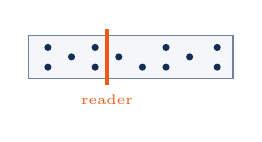
\begin{tikzpicture}
  \draw[draw=DeepBlue!60, fill=LightGray] (0,0) rectangle (2.6,0.55);
  \foreach \x/\y in {0.25/0.15,0.25/0.4,0.55/0.28,0.85/0.15,0.85/0.4,1.15/0.28,1.45/0.15,1.75/0.4,1.75/0.15,2.05/0.28,2.4/0.15,2.4/0.4}
    {\fill[DeepBlue] (\x,\y) circle (0.045);}
  \draw[AccentOrange, very thick] (1.0,-0.08) -- (1.0,0.63);
  \node[font=\tiny, text=AccentOrange, anchor=north] at (1.0,-0.08) {reader};
\end{tikzpicture}}

\newcommand{\diagMemStackSmall}{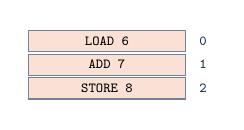
\begin{tikzpicture}
  \node[smallcell, fill=AccentOrange!18, minimum width=2.0cm] at (0,0.3) {LOAD 6};
  \node[smallcell, fill=AccentOrange!18, minimum width=2.0cm] at (0,0) {ADD 7};
  \node[smallcell, fill=AccentOrange!18, minimum width=2.0cm] at (0,-0.3) {STORE 8};
  \node[addr, font=\ttfamily\tiny, anchor=west] at (1.05,0.3) {0};
  \node[addr, font=\ttfamily\tiny, anchor=west] at (1.05,0) {1};
  \node[addr, font=\ttfamily\tiny, anchor=west] at (1.05,-0.3) {2};
\end{tikzpicture}}

\newcommand{\diagTwoMem}{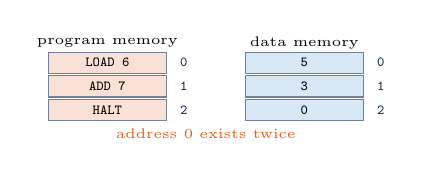
\begin{tikzpicture}
  \node[font=\tiny] at (0,0.55) {program memory};
  \node[font=\tiny] at (2.5,0.55) {data memory};
  \node[smallcell, fill=AccentOrange!18, minimum width=1.5cm] at (0,0.3) {LOAD 6};
  \node[smallcell, fill=AccentOrange!18, minimum width=1.5cm] at (0,0) {ADD 7};
  \node[smallcell, fill=AccentOrange!18, minimum width=1.5cm] at (0,-0.3) {HALT};
  \node[smallcell, fill=StorageBlue!18, minimum width=1.5cm] at (2.5,0.3) {5};
  \node[smallcell, fill=StorageBlue!18, minimum width=1.5cm] at (2.5,0) {3};
  \node[smallcell, fill=StorageBlue!18, minimum width=1.5cm] at (2.5,-0.3) {0};
  \foreach \i in {0,1,2} {
    \node[addr, font=\ttfamily\tiny, anchor=west] at (0.8,{0.3-0.3*\i}) {\i};
    \node[addr, font=\ttfamily\tiny, anchor=west] at (3.3,{0.3-0.3*\i}) {\i};
  }
  \node[font=\tiny, text=AccentOrange] at (1.25,-0.6) {address 0 exists twice};
\end{tikzpicture}}

\newcommand{\diagOneMem}{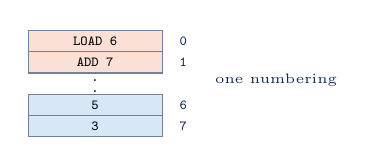
\begin{tikzpicture}
  \node[smallcell, fill=AccentOrange!18, minimum width=1.7cm] (o0) at (0,0.5) {LOAD 6};
  \node[smallcell, fill=AccentOrange!18, minimum width=1.7cm] at (0,0.23) {ADD 7};
  \node[smallcell, draw=none, minimum width=1.7cm] at (0,-0.04) {$\vdots$};
  \node[smallcell, fill=StorageBlue!18, minimum width=1.7cm] at (0,-0.31) {5};
  \node[smallcell, fill=StorageBlue!18, minimum width=1.7cm] at (0,-0.58) {3};
  \node[addr, font=\ttfamily\tiny, anchor=west] at (0.95,0.5) {0};
  \node[addr, font=\ttfamily\tiny, anchor=west] at (0.95,0.23) {1};
  \node[addr, font=\ttfamily\tiny, anchor=west] at (0.95,-0.31) {6};
  \node[addr, font=\ttfamily\tiny, anchor=west] at (0.95,-0.58) {7};
  \node[font=\tiny, text=DeepBlue, anchor=west] at (1.4,0) {one numbering};
\end{tikzpicture}}

\newcommand{\diagDecimal}{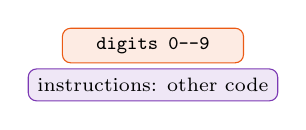
\begin{tikzpicture}
  \node[draw=AccentOrange, fill=AccentOrange!12, rounded corners=3pt, font=\ttfamily\scriptsize, minimum height=0.4cm,
    minimum width=2.3cm] at (0,0.28) {digits 0--9};
  \node[draw=ProgramPurple, fill=ProgramPurple!12, rounded corners=3pt, font=\scriptsize, minimum height=0.4cm,
    minimum width=2.3cm] at (0,-0.22) {instructions: other code};
\end{tikzpicture}}

\newcommand{\diagBinary}{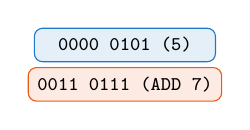
\begin{tikzpicture}
  \node[draw=StorageBlue, fill=StorageBlue!12, rounded corners=3pt, font=\ttfamily\scriptsize, minimum height=0.4cm,
    minimum width=2.3cm] at (0,0.28) {0000 0101 (5)};
  \node[draw=AccentOrange, fill=AccentOrange!12, rounded corners=3pt, font=\ttfamily\scriptsize, minimum height=0.4cm,
    minimum width=2.3cm] at (0,-0.22) {0011 0111 (ADD 7)};
\end{tikzpicture}}

\newcommand{\diagParallel}{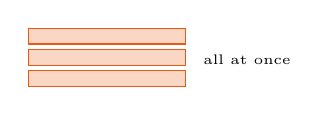
\begin{tikzpicture}
  \foreach \k in {0,1,2} {\draw[fill=AccentOrange!25, draw=AccentOrange] (0,{0.6-0.27*\k}) rectangle (2.0,{0.4-0.27*\k});}
  \node[font=\tiny, anchor=west] at (2.1,0.2) {all at once};
\end{tikzpicture}}

\newcommand{\diagDataflow}{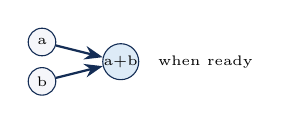
\begin{tikzpicture}[>=Stealth]
  \node[circle, draw=DeepBlue, fill=LightGray, minimum size=0.35cm, inner sep=0pt, font=\tiny] (a) at (0,0.3) {a};
  \node[circle, draw=DeepBlue, fill=LightGray, minimum size=0.35cm, inner sep=0pt, font=\tiny] (b) at (0,-0.2) {b};
  \node[circle, draw=DeepBlue, fill=StorageBlue!15, minimum size=0.4cm, inner sep=0pt, font=\tiny] (c) at (1.0,0.05) {a+b};
  \draw[->, thick, DeepBlue] (a) -- (c); \draw[->, thick, DeepBlue] (b) -- (c);
  \node[font=\tiny, anchor=west] at (1.35,0.05) {when ready};
\end{tikzpicture}}

\newcommand{\diagSequential}{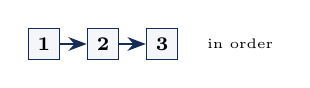
\begin{tikzpicture}[>=Stealth]
  \foreach \k in {1,2,3} {\node[draw=DeepBlue, fill=LightGray, minimum size=0.4cm, inner sep=0pt, font=\scriptsize\bfseries]
    (s\k) at ({0.75*\k-0.75},0.05) {\k};}
  \draw[->, thick, DeepBlue] (s1) -- (s2); \draw[->, thick, DeepBlue] (s2) -- (s3);
  \node[font=\tiny, anchor=west] at (1.95,0.05) {in order};
\end{tikzpicture}}

\newcommand{\diagMonolith}{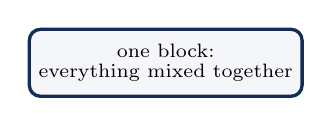
\begin{tikzpicture}
  \node[draw=DeepBlue, very thick, rounded corners=4pt, fill=LightGray, minimum width=2.6cm, minimum height=0.85cm,
    font=\scriptsize, align=center] {one block:\\[-1pt]everything mixed together};
\end{tikzpicture}}

\newcommand{\diagUnits}{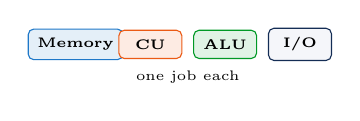
\begin{tikzpicture}
  \node[draw=StorageBlue, fill=StorageBlue!12, rounded corners=2pt, font=\tiny\bfseries, minimum width=0.8cm, minimum height=0.36cm] at (0,0.22) {Memory};
  \node[draw=AccentOrange, fill=AccentOrange!12, rounded corners=2pt, font=\tiny\bfseries, minimum width=0.8cm, minimum height=0.36cm] at (0.95,0.22) {CU};
  \node[draw=mygreen, fill=mygreen!12, rounded corners=2pt, font=\tiny\bfseries, minimum width=0.8cm, minimum height=0.36cm] at (1.9,0.22) {ALU};
  \node[draw=DeepBlue, fill=LightGray, rounded corners=2pt, font=\tiny\bfseries, minimum width=0.8cm, minimum height=0.36cm] at (2.85,0.22) {I/O};
  \node[font=\tiny] at (1.425,-0.2) {one job each};
\end{tikzpicture}}

% ---------- helpers for the CPU section ----------
\tikzset{
  reg/.style={draw=orange!80!black, very thick, fill=yellow!25, rounded corners=2pt,
    minimum width=1.95cm, minimum height=0.55cm, inner sep=2pt, font=\ttfamily\scriptsize, align=center},
  cpuunit/.style={very thick, rounded corners=3pt, minimum width=1.2cm, minimum height=0.6cm,
    inner sep=2pt, font=\scriptsize\bfseries, align=center},
  hot/.style={fill=AccentOrange!45, draw=AccentOrange, very thick},
  hotdata/.style={fill=StorageBlue!40, draw=StorageBlue, very thick},
  hotalu/.style={fill=mygreen!18, line width=1.6pt},
  fetcharrow/.style={-{Stealth}, very thick, DeepBlue, rounded corners=3pt},
  dataarrow/.style={-{Stealth}, very thick, DeepBlue, rounded corners=3pt},
  steplabel/.style={font=\tiny\bfseries, fill=white, inner sep=1pt},
}
% memory with the running example
% #1 highlighted instruction (0-3, -1 = none)  #2 text of cell 8  #3 highlighted data cell (6-8, 0 = none)
\newcommand{\mempanel}[3]{%
  \node[font=\scriptsize\bfseries, text=StorageBlue] at (0,1.8) {Memory};
  \foreach \i/\t in {0/{0001 0110\ \ LOAD 6},1/{0011 0111\ \ ADD 7},2/{0010 1000\ \ STORE 8},3/{0111 0000\ \ HALT}} {
    \ifnum\i=#1
      \node[instrcell, minimum width=2.9cm, hot] (m\i) at (0,{1.35-0.45*\i}) {\t};
    \else
      \node[instrcell, minimum width=2.9cm] (m\i) at (0,{1.35-0.45*\i}) {\t};
    \fi
    \node[addr, anchor=east] at (-1.5,{1.35-0.45*\i}) {\i};
  }
  \node[memcell, draw=none, minimum width=2.9cm] at (0,-0.45) {$\vdots$};
  \foreach \i/\t/\y in {6/{0000 0101\ \ (5)}/-0.9,7/{0000 0011\ \ (3)}/-1.35,8/{#2}/-1.8} {
    \ifnum\i=#3
      \node[datacell, minimum width=2.9cm, hotdata] (m\i) at (0,\y) {\t};
    \else
      \node[datacell, minimum width=2.9cm] (m\i) at (0,\y) {\t};
    \fi
    \node[addr, anchor=east] at (-1.5,\y) {\i};
  }
}
% the CPU, built up step by step
% #1 level: 0 empty, 1 +PC, 2 +IR, 3 +AC, 4 +ALU, 5 +CU   #2 PC   #3 IR   #4 AC   #5 extra ALU style
\newcommand{\cpupanel}[5]{%
  \node[draw=DeepBlue, very thick, rounded corners=6pt, fill=DeepBlue!6, minimum width=4.65cm,
    minimum height=3.85cm, anchor=west] (cpu) at (2.45,-0.2) {};
  \node[font=\scriptsize\bfseries, text=DeepBlue, anchor=north west] at ([shift={(0.1,-0.06)}]cpu.north west) {CPU};
  \ifnum#1>0 \node[reg] (pc) at (3.65,0.95) {\textbf{PC}\ \ #2}; \fi
  \ifnum#1>1 \node[reg] (ir) at (3.65,0.0) {\textbf{IR}\\[-1pt]#3}; \fi
  \ifnum#1>2 \node[reg] (ac) at (3.65,-1.05) {\textbf{AC}\ \ #4}; \fi
  \ifnum#1>3 \node[cpuunit, draw=mygreen, fill=mygreen!18, #5] (alu) at (6.3,-1.05)
    {\textcolor{mygreen!60!black}{\faCalculator}\\[-1pt]ALU}; \fi
  \ifnum#1>4 \node[cpuunit, draw=AccentOrange, fill=AccentOrange!18] (cu) at (6.3,0.5)
    {\textcolor{AccentOrange}{\faCogs}\\[-1pt]CU}; \fi
}
% explanation slide: #1 title, #2 tikz body (memory + CPU), #3 right-hand column
\newcommand{\explainframe}[3]{%
\begin{frame}{#1}
  \begin{columns}[c,onlytextwidth]
    \column{0.58\textwidth}
      \centering
      \begin{tikzpicture}[>=Stealth, scale=0.92, every node/.append style={transform shape}]
        #2
      \end{tikzpicture}
    \column{0.4\textwidth}
      #3
  \end{columns}
\end{frame}}
% boxes for the right-hand column
\newcommand{\defbox}[1]{%
  \begin{beamercolorbox}[rounded=true,sep=0.1cm,wd=\linewidth]{block body example}
    \footnotesize #1
  \end{beamercolorbox}\vspace{0.06cm}}
\newcommand{\stepbox}[2]{%
  \begin{beamercolorbox}[rounded=true,sep=0.09cm,wd=\linewidth]{block body}
    \footnotesize\textbf{#1}\\ #2
  \end{beamercolorbox}\vspace{0.06cm}}
\newcommand{\phasename}[1]{%
  {\centering\footnotesize Name of this phase:\ \colorbox{DeepBlue}{\textcolor{white}{\textbf{#1}}}\par}}
% small tag above the CPU box: which instruction is being executed
\newcommand{\executing}[1]{%
  \node[font=\scriptsize\bfseries, text=AccentOrange, anchor=south east] at ([yshift=1pt]cpu.north east)
    {Executing: \texttt{#1}};}
\newcommand{\statebox}[1]{%
  {\centering\scriptsize\textcolor{DeepBlue}{\textbf{State:}}\ #1\par}}

\lstset{
  language=Python,
  basicstyle=\color{VSText}\ttfamily\footnotesize,
  keywordstyle=\color{VSPurple}\bfseries,
  stringstyle=\color{VSString},
  commentstyle=\color{VSComment}\itshape,
  numbers=left,
  numberstyle=\tiny\color{gray},
  stepnumber=1,
  breaklines=true,
  showstringspaces=false,
  xleftmargin=15pt,
  xrightmargin=5pt,
  frame=none
}

% MARIE assembly: line numbers start at 0, so a line number equals the memory address
\lstdefinelanguage{MARIE}{
  morekeywords={Load,Store,Add,Subt,Input,Output,Halt,Jump,Skipcond,DEC,HEX,ADR,LoadI,StoreI,AddI,JumpI,JnS,Clear,LoadImmi},
  sensitive=false,
  comment=[l]{/},
}
\lstdefinestyle{marie}{language=MARIE, firstnumber=0, basicstyle=\color{VSText}\ttfamily\scriptsize,
  keywordstyle=\color{VSBlue}\bfseries, commentstyle=\color{VSComment}\itshape,
  columns=fixed, basewidth=0.52em, keepspaces=true, breaklines=false, xleftmargin=12pt}

\BeforeBeginEnvironment{lstlisting}{%
  \begin{beamercolorbox}[rounded=true,sep=2mm,wd=\linewidth]{vscodelisting}%
  
\begin{tikzpicture}
    \fill[MacRed] (0,0) circle (3pt);
    \fill[MacYellow] (0.35,0) circle (3pt);
    \fill[MacGreen] (0.70,0) circle (3pt);
  \end{tikzpicture}%
  \vspace{-0.2cm}%
}
\AfterEndEnvironment{lstlisting}{\end{beamercolorbox}}

% =====================================================================
%  Day 2 helpers
% =====================================================================

% ---------- MARIE datapath, drawn like the Data Path view of MARIE.js ----------
% \busdiagram[values]{source}{destination}{extra TikZ}
%   source (Read, blue) and destination (Write, red): ir, out, in, ac, mbr, pc, mar, mem, none
%   values: ir=, out=, in=, ac=, mbr=, pc=, mar=, mem= (contents of M[MAR]), step= (0-7, -1 = none)
\definecolor{ReadBlue}{RGB}{30,150,230}
\definecolor{WriteRed}{RGB}{220,50,80}
\definecolor{BusGreen}{RGB}{60,170,110}
\tikzset{
  dpreg/.style={draw=DeepBlue!80, thick, fill=white, minimum width=1.1cm, minimum height=0.46cm,
    inner sep=1pt, font=\ttfamily\scriptsize},
  dpname/.style={font=\tiny, text=DeepBlue!80, above=0pt, inner sep=1pt},
  dpwire/.style={thin, DeepBlue!18},
  dpmem/.style={draw=StorageBlue, very thick, fill=StorageBlue!12, rounded corners=3pt,
    minimum width=1.3cm, minimum height=0.95cm, font=\scriptsize\bfseries, align=center},
  srcreg/.style={draw=ReadBlue, line width=1.6pt},
  dstreg/.style={draw=WriteRed, line width=1.6pt},
}
\pgfkeys{/dp/.is family, /dp,
  ir/.initial={0000}, out/.initial={0000}, in/.initial={0000}, ac/.initial={0000},
  mbr/.initial={0000}, pc/.initial={000}, mar/.initial={000}, mem/.initial={0000},
  step/.initial={-1}}
\newcommand{\dpv}[1]{\pgfkeysvalueof{/dp/#1}}
\newcommand{\busdiagram}[4][]{%
  \begingroup
  \pgfkeys{/dp, ir=0000, out=0000, in=0000, ac=0000, mbr=0000, pc=000, mar=000, mem=0000, step=-1, #1}%
  \begin{tikzpicture}[>=Stealth]
    \tikzset{bd-mem/.style={}, bd-mar/.style={}, bd-pc/.style={}, bd-mbr/.style={},
      bd-ac/.style={}, bd-ir/.style={}, bd-in/.style={}, bd-out/.style={}, bd-none/.style={}}
    \tikzset{bd-#2/.style={srcreg}}
    \tikzset{bd-#3/.style={dstreg}}
    % ----- control unit -----
    \node[draw=DeepBlue!80, thick, fill=white, minimum width=1.3cm, minimum height=2.95cm,
      anchor=north west] (cu) at (-2.4,2.0) {};
    \node[font=\tiny, text=DeepBlue, anchor=north west, below=1pt] at (cu.south west) {Control unit};
    \node[font=\tiny, text=DeepBlue!80, anchor=east] at (-1.15,1.75) {Read};
    \node[font=\tiny, text=DeepBlue!80, anchor=east] at (-1.15,-0.6) {Write};
    \node[font=\tiny, text=DeepBlue!80, anchor=east] at (-1.15,0.05) {AC<0};
    \node[font=\tiny, text=DeepBlue!80, anchor=east] at (-1.15,-0.15) {AC=0};
    \node[font=\tiny, text=DeepBlue!80] at (-2.0,1.3) {Step};
    \foreach \k in {0,...,7} {
      \pgfmathtruncatemacro{\cur}{\dpv{step}}
      \ifnum\k=\cur
        \fill[ReadBlue] (-2.0,{1.1-0.15*\k}) circle (0.065);
      \else
        \fill[DeepBlue!30] (-2.0,{1.1-0.15*\k}) circle (0.035);
      \fi
    }
    % ----- memory -----
    \node[draw=DeepBlue!80, thick, fill=white, minimum width=1.5cm, minimum height=2.95cm,
      anchor=north west, bd-mem] (mem) at (10.4,2.0) {};
    \node[font=\tiny, text=DeepBlue, anchor=north west, below=1pt] at (mem.south west) {Main memory};
    \node[font=\ttfamily\tiny, text=DeepBlue!80] at (11.15,0.75) {M[MAR]};
    \node[font=\ttfamily\scriptsize] at (11.15,0.5) {\dpv{mem}};
    % ----- faint control wires (one Read and one Write wire per device) -----
    \draw[dpwire] (-1.1,1.75) -- (10.4,1.75);
    \draw[dpwire] (-1.1,-0.6) -- (10.4,-0.6);
    \foreach \x in {0.6,2.0,3.4,4.8,6.2,7.6,9.0} {
      \draw[dpwire] (\x-0.25,1.75) -- (\x-0.25,1.18);
      \draw[dpwire] (\x+0.3,-0.6) -- (\x+0.3,0.72);
    }
    % ----- bus (drawn first, registers on top) -----
    \foreach \x in {0.6,2.0,3.4,4.8,6.2,7.6,9.0}
      \draw[line width=2.6pt, BusGreen] (\x,0.72) -- (\x,-0.35);
    \draw[line width=2.6pt, BusGreen] (0.6-0.045,-0.35) -- (10.4,-0.35);
    % ----- ALU between AC and MBR, with its links and the flag wires to the CU -----
    \draw[thin, DeepBlue!40] (4.45,0.05) -- (-1.1,0.05);
    \draw[thin, DeepBlue!40] (4.45,-0.15) -- (-1.1,-0.15);
    \draw[thick, DeepBlue!70, fill=white] (5.0,0.47) -- (5.42,0.47) -- (5.5,0.37) -- (5.58,0.47) -- (6.0,0.47)
      -- (5.72,0.05) -- (5.28,0.05) -- cycle;
    \node[font=\tiny, text=DeepBlue!80] at (5.5,0.22) {ALU};
    \draw[thick, DeepBlue!60] (5.2,0.72) -- (5.2,0.47);
    \draw[thick, DeepBlue!60] (5.8,0.72) -- (5.8,0.47);
    \draw[thick, DeepBlue!60] (5.5,0.05) -- (5.5,-0.1) -- (4.45,-0.1) |- (4.45,0.72);
    % ----- registers -----
    \foreach \n/\x/\lab in {ir/0.6/IR, out/2.0/OUT, in/3.4/IN, ac/4.8/AC, mbr/6.2/MBR, pc/7.6/PC, mar/9.0/MAR} {
      \node[dpreg, bd-\n] (\n) at (\x,0.95) {\dpv{\n}};
      \node[dpname] at (\n.north) {\lab};
      \coordinate (\n-port) at (\n.south);
      \coordinate (\n-bus) at (\x,-0.35);
    }
    \coordinate (mem-port) at (10.4,-0.35);
    \coordinate (mem-bus) at (10.4,-0.35);
    % IR is decoded by the CU; MAR selects the memory cell
    \draw[thick, BusGreen, -{Stealth}] (ir.west) -- (-1.1,0.95);
    \draw[thick, BusGreen, -{Stealth}] (mar.east) -- (10.4,0.95);
    % ----- active Read and Write signals -----
    \ifstrequal{#2}{none}{}{%
      \ifstrequal{#2}{mem}
        {\draw[line width=1.3pt, ReadBlue, -{Stealth}] (-1.1,1.75) -- (10.4,1.75);}
        {\draw[line width=1.3pt, ReadBlue, -{Stealth}] (-1.1,1.75) -| ($(#2.north)+(-0.25,0)$);}}
    \ifstrequal{#3}{none}{}{%
      \ifstrequal{#3}{mem}
        {\draw[line width=1.3pt, WriteRed, -{Stealth}] (-1.1,-0.6) -- (10.4,-0.6);}
        {\draw[line width=1.3pt, WriteRed, -{Stealth}] (-1.1,-0.6) -| ($(#3.south)+(0.3,0)$);}}
    % ----- the value travelling along the bus -----
    \ifstrequal{#2}{none}{}{\ifstrequal{#3}{none}{}{%
      \draw[line width=3pt, BusGreen] (#2-port) -- (#2-bus) -- (#3-bus) -- (#3-port);
      \draw[line width=1.5pt, white, dash pattern=on 1.5pt off 1.5pt] (#2-port) -- (#2-bus) -- (#3-bus) -- (#3-port);}}
    #4
  \end{tikzpicture}%
  \endgroup}

% legend for the colours of the data path
\newcommand{\dplegend}{%
  {\tiny\textcolor{ReadBlue}{\rule{0.25cm}{0.2cm}}\ \textbf{Read}: puts its value on the bus
  \qquad\textcolor{WriteRed}{\rule{0.25cm}{0.2cm}}\ \textbf{Write}: stores the value from the bus
  \qquad\tikz[baseline=-0.6ex]{\draw[line width=3pt, BusGreen] (0,0) -- (0.5,0);\draw[line width=1.5pt, white, dash pattern=on 1.5pt off 1.5pt] (0,0) -- (0.5,0);}\ the value travelling on the bus}}

% one step of an instruction: data path on top, explanation below
% #1 title, #2 source, #3 destination, #4 values (keys), #5 explanation
\newcommand{\stepframe}[5]{%
\begin{frame}{#1}
  \begin{center}
    \resizebox{0.8\textwidth}{!}{\busdiagram[#4]{#2}{#3}{}}\\[0.02cm]
    \dplegend
  \end{center}
  \vspace{-0.1cm}
  \begin{center}
    \begin{minipage}{0.8\textwidth}
      #5
    \end{minipage}
  \end{center}
\end{frame}}

% ---------- timeline of clock steps ----------
% #1 fetch steps, #2 execute steps, #3 label on the right
\newcommand{\steptimeline}[3]{%
  \begin{tikzpicture}
    \foreach \i in {1,...,#1}
      \node[draw=white, fill=StorageBlue!75, text=white, font=\tiny\bfseries, minimum width=0.62cm,
        minimum height=0.45cm, inner sep=0pt] at ({0.62*(\i-1)},0) {T\the\numexpr\i-1\relax};
    \foreach \i in {1,...,#2}
      \node[draw=white, fill=AccentOrange, text=white, font=\tiny\bfseries, minimum width=0.62cm,
        minimum height=0.45cm, inner sep=0pt] at ({0.62*(#1+\i-1)},0) {T\the\numexpr#1+\i-1\relax};
    \node[anchor=west, font=\scriptsize] at ({0.62*(#1+#2)-0.25},0) {#3};
  \end{tikzpicture}}

% legend for the timeline colours
\newcommand{\timelinelegend}{%
  {\tiny\textcolor{StorageBlue!75}{\rule{0.25cm}{0.2cm}}\ fetch
  \qquad\textcolor{AccentOrange}{\rule{0.25cm}{0.2cm}}\ execute}}

% ---------- small pieces for the addressing-mode slides ----------
\tikzset{
  mcell/.style={draw=DeepBlue!60, minimum width=1.5cm, minimum height=0.42cm, inner sep=1pt,
    font=\ttfamily\scriptsize, align=center, fill=StorageBlue!15},
  mcellhot/.style={mcell, fill=StorageBlue!45, draw=StorageBlue, very thick},
  mcellptr/.style={mcell, fill=ProgramPurple!18, draw=ProgramPurple, very thick},
  instrbox/.style={draw=AccentOrange, very thick, fill=AccentOrange!15, rounded corners=2pt,
    minimum height=0.5cm, inner sep=3pt, font=\ttfamily\scriptsize},
  ptrarrow/.style={-{Stealth}, very thick, DeepBlue},
  valarrow/.style={-{Stealth}, very thick, DeepBlue},
}

% task header box (same look as on Day 1)
% #1 form and time, #2 short instruction
\newcommand{\taskhead}[2]{%
  \begin{beamercolorbox}[rounded=true,sep=0.12cm,wd=\linewidth]{block body example}
    \small\textbf{#1}\\[0.04cm]
    \footnotesize #2
  \end{beamercolorbox}\vspace{0.1cm}}

% highlighted key message at the bottom of a slide
\newcommand{\keymsg}[1]{%
  \begin{beamercolorbox}[rounded=true,sep=0.1cm,wd=\textwidth]{block body example}
    \centering\footnotesize #1
  \end{beamercolorbox}}

% register transfer written in text: \mo{MAR}{PC} gives MAR <- PC
\newcommand{\mo}[2]{\texttt{#1\,$\leftarrow$\,#2}}

% plain listings (x86, RISC-V) without Python highlighting
\lstdefinelanguage{plain}{}
\lstdefinestyle{asm}{language=plain, basicstyle=\color{VSText}\ttfamily\scriptsize, numbers=none,
  columns=fixed, basewidth=0.52em, keepspaces=true, xleftmargin=6pt}

% =====================================================================
%  Day 3 helpers
% =====================================================================

\usetikzlibrary{patterns}
\usepackage{multirow}
% ---------- RISC-V listings ----------
\lstdefinestyle{rv}{language=RISCV, basicstyle=\color{VSText}\ttfamily\scriptsize, numbers=none,
  keywordstyle=\color{VSBlue}\bfseries, keywordstyle={[2]\color{VSPurple}\bfseries},
  commentstyle=\color{VSComment}\itshape,
  columns=fixed, basewidth=0.52em, keepspaces=true, breaklines=false, xleftmargin=6pt}
\lstdefinestyle{rvnum}{style=rv, numbers=left, firstnumber=1, xleftmargin=14pt}

% ---------- colours of the five pipeline stages (the same all day) ----------
\colorlet{cIF}{AccentOrange}
\colorlet{cID}{ProgramPurple}
\colorlet{cEX}{mygreen}
\colorlet{cMEM}{StorageBlue}
\colorlet{cWB}{DeepBlue}

% ---------- pipeline diagrams ----------
% cell size (cm)
\def\pw{0.74}
\def\ph{0.46}
\tikzset{
  pcell/.style={minimum width=\pw cm, minimum height=\ph cm, inner sep=0pt, draw=white,
    font=\scriptsize\bfseries, text=white},
  pst-IF/.style={pcell, fill=cIF},
  pst-ID/.style={pcell, fill=cID},
  pst-EX/.style={pcell, fill=cEX},
  pst-MEM/.style={pcell, fill=cMEM},
  pst-WB/.style={pcell, fill=cWB},
  pst-B/.style={pcell, fill=gray!25, text=gray!70, font=\tiny},
  pst-X/.style={pcell, fill=MacRed!20, text=MacRed},
  pst-N/.style={pcell, fill=none, draw=none},
  pst-E/.style={pcell, fill=gray!10},
  plab/.style={anchor=east, font=\ttfamily\footnotesize, inner sep=1pt},
}
% one row of a pipeline diagram
% #1 row (0 = top), #2 first cycle (1-based), #3 comma list of IF, ID, EX, MEM, WB, B (bubble), X (flushed), N (empty)
\newcommand{\prow}[3]{%
  \foreach \s [count=\k from 0] in {#3} {%
    \node[pst-\s] at ({(#2+\k-1)*\pw}, {-(#1)*\ph}) {%
      \expandafter\ifstrequal\expandafter{\s}{B}{bubble}{%
      \expandafter\ifstrequal\expandafter{\s}{X}{$\times$}{%
      \expandafter\ifstrequal\expandafter{\s}{N}{}{\expandafter\ifstrequal\expandafter{\s}{E}{}{\s}}}}};
  }}
% label of a row
\newcommand{\plabel}[2]{\node[plab] at ({-0.5*\pw-0.05}, {-(#1)*\ph}) {#2};}
% cycle numbers above the diagram: #1 number of cycles
\newcommand{\pcycles}[1]{%
  \foreach \c in {1,...,#1}
    \node[font=\scriptsize, text=DeepBlue!70] at ({(\c-1)*\pw}, {0.8*\ph}) {\c};
  \node[font=\scriptsize, text=DeepBlue!70, anchor=east] at ({-0.5*\pw-0.05}, {0.8*\ph}) {cycle};}
% highlight one column: #1 cycle, #2 number of rows, #3 colour
\newcommand{\pcolumn}[3]{%
  \draw[#3, very thick, rounded corners=2pt]
    ({(#1-1.5)*\pw}, {0.5*\ph}) rectangle ({(#1-0.5)*\pw}, {-(#2-0.5)*\ph});}

% legend of stage colours
\newcommand{\stagelegend}{%
  {\tiny
  \textcolor{cIF}{\rule{0.25cm}{0.2cm}}\,IF fetch\quad
  \textcolor{cID}{\rule{0.25cm}{0.2cm}}\,ID decode\quad
  \textcolor{cEX}{\rule{0.25cm}{0.2cm}}\,EX execute\quad
  \textcolor{cMEM}{\rule{0.25cm}{0.2cm}}\,MEM memory\quad
  \textcolor{cWB}{\rule{0.25cm}{0.2cm}}\,WB write back}}

% ---------- stage boxes ----------
\tikzset{
  stagebox/.style={very thick, rounded corners=4pt, minimum width=1.9cm, minimum height=0.8cm,
    align=center, font=\small\bfseries, drop shadow},
  gbar/.style={minimum height=0.36cm, inner sep=0pt, draw=white, font=\tiny\bfseries, text=white},
  gempty/.style={minimum height=0.36cm, inner sep=0pt, draw=gray!50, dashed, font=\tiny, text=gray!60},
  unit/.style={draw=DeepBlue, very thick, fill=white, rounded corners=3pt, align=center,
    font=\scriptsize\bfseries, inner sep=2pt},
}

% ---------- a simple RISC-V datapath ----------
% #1 extra TikZ drawn on top (nodes: pc, imem, rf, alu, dmem, mux, cu, add4)
\newcommand{\rvdatapath}[1]{%
  \begin{tikzpicture}[>=Stealth, font=\scriptsize]
    % stage labels
    \foreach \x/\n/\c in {0.9/IF/cIF, 4.2/ID/cID, 6.6/EX/cEX, 9.0/MEM/cMEM, 10.9/WB/cWB}
      \node[fill=\c, text=white, rounded corners=2pt, font=\tiny\bfseries, minimum width=0.9cm] at (\x,2.35) {\n};
    % units
    \node[unit, minimum width=0.6cm, minimum height=1.0cm] (pc) at (0,0) {PC};
    \node[unit, minimum width=1.5cm, minimum height=1.6cm] (imem) at (1.8,0) {Instruction\\memory};
    \node[unit, minimum width=1.5cm, minimum height=1.8cm] (rf) at (4.2,0) {Register\\file};
    \draw[DeepBlue, very thick, fill=white] (6.2,0.9) -- (7.0,0.45) -- (7.0,-0.45) -- (6.2,-0.9) -- (6.2,-0.25)
      -- (6.4,0) -- (6.2,0.25) -- cycle;
    \node[font=\scriptsize\bfseries] (alu) at (6.68,0) {ALU};
    \coordinate (aluin1) at (6.2,0.55); \coordinate (aluin2) at (6.2,-0.55); \coordinate (aluout) at (7.0,0);
    \node[unit, minimum width=1.5cm, minimum height=1.6cm] (dmem) at (9.0,0) {Data\\memory};
    \node[unit, minimum width=0.45cm, minimum height=1.2cm, rounded corners=6pt, font=\tiny] (mux) at (10.9,0) {M\\U\\X};
    \node[unit, minimum width=1.3cm, minimum height=0.5cm, draw=DeepBlue!60, text=DeepBlue!80] (add4) at (0.9,1.55) {$+4$};
    \node[unit, minimum width=2.2cm, minimum height=0.5cm, draw=gray, text=gray] (cu) at (4.2,-1.85) {Control unit};
    % wires
    \draw[->, thick] (pc) -- (imem);
    \draw[->, thick] (imem) -- node[above, font=\tiny] {instruction} (rf);
    \draw[->, thick] ([yshift=0.55cm]rf.east) -- (aluin1);
    \draw[->, thick] ([yshift=-0.55cm]rf.east) -- (aluin2);
    \draw[->, thick] (aluout) -- node[above, font=\tiny] {address} ([yshift=0cm]dmem.west);
    \draw[->, thick] ([yshift=-0.55cm]dmem.east) -- ([yshift=-0.4cm]mux.west);
    \draw[->, thick] (7.3,0) |- (7.3,-1.1) -| (10.3,-1.1) |- ([yshift=0.4cm]mux.west);
    \draw[->, thick] (mux.east) -- ++(0.3,0) |- (11.2,2.0) -| node[pos=0.25, above, font=\tiny] {write back} (4.2,0.9);
    \draw[->, thick, DeepBlue!60] (pc.north) |- (add4.west);
    \draw[->, thick, DeepBlue!60] (add4.east) -- ++(0.35,0) |- (-0.6,1.95) |- (pc.west);
    \draw[->, dashed, gray] (cu.north) -- (rf.south);
    \draw[->, dashed, gray] (cu.east) -| (dmem.south);
    \draw[->, dashed, gray] (cu.east) -| (mux.south);
    #1
  \end{tikzpicture}}

% ---------- Ripes window (schematic; replace with a real screenshot if you like) ----------
\newcommand{\ripeswindow}{%
  \begin{tikzpicture}[font=\tiny]
    \draw[DeepBlue, very thick, fill=white, rounded corners=4pt] (0,0) rectangle (9,5.4);
    \fill[DeepBlue!10, rounded corners=4pt] (0,5.0) rectangle (9,5.4);
    \fill[MacRed] (0.25,5.2) circle (2.5pt); \fill[MacYellow] (0.5,5.2) circle (2.5pt); \fill[MacGreen] (0.75,5.2) circle (2.5pt);
    \node[font=\tiny\bfseries, text=DeepBlue] at (4.5,5.2) {Ripes};
    % toolbar
    \fill[LightGray] (0,4.55) rectangle (9,5.0);
    \foreach \x/\i in {1.0/\faMicrochip, 1.6/\faStepForward, 2.2/\faPlay, 2.8/\faFastForward, 3.4/\faUndo}
      \node[text=DeepBlue] at (\x,4.77) {\i};
    % side bar
    \fill[DeepBlue!85] (0,0) rectangle (0.5,4.55);
    \foreach \y/\i in {4.1/\faEdit, 3.5/\faMicrochip, 2.9/\faMemory, 2.3/\faTerminal}
      \node[text=white] at (0.25,\y) {\i};
    % editor
    \draw[gray!60, fill=VSDarkBg] (0.65,0.15) rectangle (3.2,4.4);
    \foreach \y/\t in {4.1/lw x5{,} X, 3.8/lw x6{,} Y, 3.5/add x7{,} x5{,} x6, 3.2/addi x7{,} x7{,} -2, 2.9/sw x7{,} Z{,} x28}
      \node[anchor=west, text=VSText, font=\ttfamily\tiny] at (0.75,\y) {\t};
    % processor view
    \draw[gray!60, fill=LightGray] (3.35,1.4) rectangle (7.3,4.4);
    \foreach \x/\c in {3.8/cIF, 4.5/cID, 5.3/cEX, 6.1/cMEM, 6.8/cWB}
      \draw[\c, very thick, fill=\c!15] (\x-0.25,2.3) rectangle (\x+0.25,3.6);
    \draw[->, thick, DeepBlue!60] (3.55,2.95) -- (7.05,2.95);
    \node[font=\tiny, text=DeepBlue] at (5.3,1.85) {datapath};
    % statistics
    \draw[gray!60, fill=white] (3.35,0.15) rectangle (7.3,1.25);
    \node[anchor=west, font=\tiny] at (3.45,0.95) {Cycles: 13};
    \node[anchor=west, font=\tiny] at (3.45,0.7) {Instrs. retired: 8};
    \node[anchor=west, font=\tiny] at (3.45,0.45) {CPI: 1.63 \quad IPC: 0.62};
    % registers
    \draw[gray!60, fill=white] (7.45,0.15) rectangle (8.85,4.4);
    \foreach \k [count=\j from 0] in {x5,x6,x7,x8,x9,x10}
      \node[anchor=west, font=\ttfamily\tiny] at (7.5,{4.1-0.3*\j}) {\k};
    \node[font=\tiny, text=DeepBlue] at (8.15,2.1) {registers};
    % badges
    \node[circle, fill=AccentOrange, text=white, font=\bfseries\scriptsize, inner sep=1.5pt] at (1.9,1.2) {1};
    \node[circle, fill=AccentOrange, text=white, font=\bfseries\scriptsize, inner sep=1.5pt] at (1.35,4.77) {2};
    \node[circle, fill=AccentOrange, text=white, font=\bfseries\scriptsize, inner sep=1.5pt] at (5.3,4.1) {3};
    \node[circle, fill=AccentOrange, text=white, font=\bfseries\scriptsize, inner sep=1.5pt] at (6.95,0.7) {4};
    \node[circle, fill=AccentOrange, text=white, font=\bfseries\scriptsize, inner sep=1.5pt] at (8.15,1.4) {5};
  \end{tikzpicture}}

% small orange number used in running text
\newcommand{\badge}[1]{\tikz[baseline=(b.base)]\node[circle,fill=AccentOrange,text=white,
  inner sep=1.2pt,font=\bfseries\tiny] (b) {#1};}

% =====================================================================
%  Day 4 helpers
% =====================================================================

% ---------- colours of the memory levels (the same all day) ----------
\colorlet{cReg}{AccentOrange}
\colorlet{cCache}{ProgramPurple}
\colorlet{cRAM}{StorageBlue}
\colorlet{cDisk}{DeepBlue!65}
\colorlet{cIO}{mygreen}
\definecolor{HitGreen}{RGB}{39,160,70}
\colorlet{MissRed}{MacRed}
\setbeamercolor{block body answer}{bg=mygreen!10,fg=black}

% ---------- listings ----------
% RISC-V: the Day 3 keywords plus the new ones used today
\lstdefinelanguage{RISCV}{
  morekeywords={lw,sw,add,addi,sub,beq,bne,bnez,beqz,la,li,auipc,nop,ecall},
  morekeywords=[2]{.data,.text,.word,.zero},
  alsoletter={.},
  sensitive=true,
  morecomment=[l]{\#},
}
% C (for the locality examples)
\lstdefinestyle{cc}{language=C, basicstyle=\color{VSText}\ttfamily\scriptsize, numbers=none,
  keywordstyle=\color{VSBlue}\bfseries, commentstyle=\color{VSComment}\itshape,
  columns=fixed, basewidth=0.52em, keepspaces=true, breaklines=false, xleftmargin=6pt,
  moredelim=**[is][\color{MacYellow}\bfseries]{@}{@}}

% ---------- boxes for the memory levels and devices ----------
\tikzset{
  lbox/.style={very thick, rounded corners=4pt, align=center, font=\scriptsize\bfseries, inner sep=3pt},
  cpubox/.style={lbox, draw=DeepBlue, fill=DeepBlue, text=white},
  regbox/.style={lbox, draw=cReg, fill=cReg!15},
  cachebox/.style={lbox, draw=cCache, fill=cCache!12},
  rambox/.style={lbox, draw=cRAM, fill=cRAM!12},
  diskbox/.style={lbox, draw=cDisk, fill=cDisk!15},
  iobox/.style={lbox, draw=cIO, fill=cIO!12},
  dmabox/.style={lbox, draw=AccentOrange, fill=AccentOrange!12},
  osbox/.style={lbox, draw=ProgramPurple, fill=ProgramPurple!10},
  greybox/.style={lbox, draw=gray, fill=gray!8, text=gray!40!black},
  arr/.style={-{Stealth}, very thick, DeepBlue},
  okarr/.style={-{Stealth}, very thick, HitGreen},
  badarr/.style={-{Stealth}, very thick, MissRed},
  smalltxt/.style={font=\tiny, inner sep=1pt},
}

% ---------- design question box (as on the Day 1 dilemma slides) ----------
\newcommand{\designq}[1]{%
  \begin{beamercolorbox}[rounded=true,sep=0.14cm,wd=\textwidth]{block body}
    \centering\small\textbf{Design question:} #1
  \end{beamercolorbox}}
\newcommand{\whichone}{%
  {\centering\small\textcolor{DeepBlue}{\textbf{Which would you choose, and why?}}\par}}

% ---------- question card and answer card ----------
% #1 icon, #2 text
\newcommand{\qcard}[2]{%
  \begin{beamercolorbox}[rounded=true,sep=0.14cm,wd=\linewidth]{block body}
    \centering{\Large\textcolor{AccentOrange}{#1}}\\[0.12cm]
    \footnotesize #2
  \end{beamercolorbox}}
% #1 title, #2 text
\newcommand{\acard}[2]{%
  \begin{beamercolorbox}[rounded=true,sep=0.1cm,wd=\linewidth]{block body answer}
    \footnotesize\textbf{\textcolor{mygreen!70!black}{\faCheck}\ #1}\\ #2
  \end{beamercolorbox}\vspace{0.06cm}}
% red "problem" box
\setbeamercolor{block body problem}{bg=MacRed!10,fg=black}
\newcommand{\probbox}[2]{%
  \begin{beamercolorbox}[rounded=true,sep=0.09cm,wd=\linewidth]{block body problem}
    \footnotesize\textbf{\textcolor{MacRed}{\faExclamationTriangle}\ #1}\\ #2
  \end{beamercolorbox}\vspace{0.06cm}}

% ---------- hits and misses ----------
\def\cw{0.62}
\def\chh{0.42}
\tikzset{
  hmcell/.style={minimum width=\cw cm, minimum height=\chh cm, inner sep=0pt, draw=white,
    font=\scriptsize\bfseries, text=white},
  hm-H/.style={hmcell, fill=HitGreen},
  hm-M/.style={hmcell, fill=MissRed},
  hm-Q/.style={hmcell, fill=gray!10, draw=gray!40, text=gray!60},
  hm-A/.style={hmcell, draw=none, text=DeepBlue, font=\scriptsize\ttfamily\bfseries},
}
% one row of hits and misses: #1 row (0 = top), #2 comma list of H, M, Q (Q = to fill in)
\newcommand{\hmrow}[2]{%
  \foreach \s [count=\k from 0] in {#2} {%
    \node[hm-\s] at ({\k*\cw}, {-(#1)*\chh}) {\expandafter\ifstrequal\expandafter{\s}{Q}{?}{\s}};}}
% the accessed addresses above a row: #1 row, #2 comma list
\newcommand{\hmhead}[2]{%
  \foreach \s [count=\k from 0] in {#2}
    \node[hm-A] at ({\k*\cw}, {-(#1)*\chh}) {\s};}
% label on the left of a row: #1 row, #2 text
\newcommand{\hmlabel}[2]{\node[anchor=east, font=\scriptsize, inner sep=1pt] at ({-0.5*\cw-0.08}, {-(#1)*\chh}) {#2};}
% label on the right of a row: #1 row, #2 number of cells, #3 text
\newcommand{\hmresult}[3]{\node[anchor=west, font=\scriptsize\bfseries, text=DeepBlue, inner sep=1pt]
  at ({(#2-0.5)*\cw+0.12}, {-(#1)*\chh}) {#3};}

% ---------- a small cache (or page table) drawn as a table ----------
\tikzset{
  ctab/.style={draw=DeepBlue!50, minimum height=0.4cm, inner sep=1pt, font=\ttfamily\scriptsize, fill=white},
  ctabh/.style={ctab, fill=DeepBlue, text=white, font=\scriptsize\bfseries},
  ctabhit/.style={fill=HitGreen!25, draw=HitGreen, very thick},
  ctabmiss/.style={fill=MissRed!20, draw=MissRed, very thick},
}
% #1 comma list of line/valid/tag/data ; columns: Line, V, Tag, Data (top-left corner at the origin)
\newcommand{\cachetable}[1]{%
  \node[ctabh, minimum width=0.9cm] at (0,0) {Line};
  \node[ctabh, minimum width=0.7cm] at (0.8,0) {V};
  \node[ctabh, minimum width=1.0cm] at (1.65,0) {Tag};
  \node[ctabh, minimum width=1.6cm] at (2.95,0) {Data};
  \foreach \xa/\xb/\xc/\xd [count=\k from 1] in {#1} {
    \node[ctab, minimum width=0.9cm] (cl\k) at (0,{-0.4*\k}) {\xa};
    \node[ctab, minimum width=0.7cm] (cv\k) at (0.8,{-0.4*\k}) {\xb};
    \node[ctab, minimum width=1.0cm] (ct\k) at (1.65,{-0.4*\k}) {\xc};
    \node[ctab, minimum width=1.6cm] (cd\k) at (2.95,{-0.4*\k}) {\xd};
  }}

% ---------- timelines (polling, interrupts, DMA, bus use) ----------
% #1 y, #2 label on the left, #3 comma list of length/colour/text
\newcommand{\tlbar}[3]{%
  \node[anchor=east, font=\scriptsize\bfseries, text=DeepBlue, align=right] at (-0.1,#1) {#2};
  \gdef\tlx{0}%
  \foreach \tlw/\tlc/\tlt in {#3} {%
    \node[draw=white, fill=\tlc, minimum width=\tlw cm, minimum height=0.42cm, inner sep=0pt,
      anchor=west, font=\tiny\bfseries, text=white] at (\tlx,#1) {\tlt};
    \pgfmathsetmacro{\tlnext}{\tlx+\tlw}%
    \xdef\tlx{\tlnext}%
  }}

% ---------- timing diagrams (buses) ----------
% a digital signal: #1 y, #2 label, #3 comma list of x/level pairs (level 0 or 1), #4 end x
\newcommand{\signal}[4]{%
  \node[anchor=east, font=\scriptsize\bfseries, text=DeepBlue] at (-0.15,{#1+0.2}) {#2};
  \gdef\sgx{0}\gdef\sgl{0}%
  \foreach \sx/\sl in {#3} {%
    \draw[very thick, DeepBlue] (\sgx,{#1+0.4*\sgl}) -- (\sx,{#1+0.4*\sgl}) -- (\sx,{#1+0.4*\sl});
    \xdef\sgx{\sx}\xdef\sgl{\sl}%
  }
  \draw[very thick, DeepBlue] (\sgx,{#1+0.4*\sgl}) -- (#4,{#1+0.4*\sgl});}
% a bus value (address, data): #1 y, #2 label, #3 start x, #4 end x, #5 text, #6 colour
\newcommand{\busval}[6]{%
  \node[anchor=east, font=\scriptsize\bfseries, text=DeepBlue, align=right] at (-0.15,{#1+0.2}) {#2};
  \fill[#6!20] (#3,#1+0.2) -- (#3+0.12,#1+0.4) -- (#4-0.12,#1+0.4) -- (#4,#1+0.2)
    -- (#4-0.12,#1) -- (#3+0.12,#1) -- cycle;
  \draw[very thick, #6] (#3,#1+0.2) -- (#3+0.12,#1+0.4) -- (#4-0.12,#1+0.4) -- (#4,#1+0.2)
    -- (#4-0.12,#1) -- (#3+0.12,#1) -- cycle;
  \node[font=\tiny\bfseries, text=#6!70!black] at ({(#3+#4)/2},{#1+0.2}) {#5};}
% a clock: #1 y, #2 number of periods, #3 period width
\newcommand{\clocksig}[3]{%
  \node[anchor=east, font=\scriptsize\bfseries, text=DeepBlue] at (-0.15,{#1+0.2}) {Bus clock};
  \foreach \c in {1,...,#2} {
    \draw[very thick, DeepBlue] ({(\c-1)*#3},#1) -- ({(\c-1)*#3},{#1+0.4}) -- ({(\c-0.5)*#3},{#1+0.4})
      -- ({(\c-0.5)*#3},#1) -- ({\c*#3},#1);
  }}
% a vertical time marker: #1 x, #2 top y, #3 bottom y, #4 label
\newcommand{\tmark}[4]{%
  \draw[DeepBlue!50, dashed, thick] (#1,#2) -- (#1,#3);
  \node[font=\scriptsize\bfseries, text=AccentOrange, below] at (#1,#3) {#4};}

% ---------- latency bar on a log scale ----------
% #1 row, #2 label, #3 length (cm), #4 colour, #5 text at the end
\newcommand{\latbar}[5]{%
  \node[anchor=east, font=\scriptsize] at (-0.1,{-0.42*#1}) {#2};
  \fill[#4] (0,{-0.42*#1-0.15}) rectangle (#3,{-0.42*#1+0.15});
  \node[anchor=west, font=\scriptsize\bfseries, text=#4!80!black] at (#3+0.05,{-0.42*#1}) {#5};}

\title{Computer Hardware}
\subtitle{Memory and Cache}
\author{Ksawery Możdżyński}
\date{}

% ---------- the course simulators: ksawerym.github.io/ComputerHardwareSimulators ----------
\newcommand{\simbase}{https://ksawerym.github.io/ComputerHardwareSimulators/}
\newcommand{\simlink}[1]{\href{\simbase\##1}{\texttt{ksawerym.github.io/ComputerHardwareSimulators/\##1}}}
% the address of a simulator topic, shown at the bottom of a slide
\newcommand{\simfoot}[1]{\par\vfill{\hfill\scriptsize\textcolor{gray}{\faLink\ #1}\par}}

\begin{document}

\begin{frame}
  \titlepage
\end{frame}

\begin{frame}{Agenda For Today}
  \begin{columns}[T,onlytextwidth]
    \column{0.5\textwidth}
      \large
      \begin{itemize}
        \item[\textcolor{AccentOrange}{\faLayerGroup}] \textbf{1. The Memory Wall} \\
        \textcolor{gray}{\small Why memory cannot be fast \emph{and} cheap}
      \end{itemize}
    \column{0.5\textwidth}
      \large
      \begin{itemize}
        \item[\textcolor{AccentOrange}{\faBolt}] \textbf{2. Cache} \\
        \textcolor{gray}{\small Locality, hits and misses, mapping, AMAT}
      \end{itemize}
  \end{columns}
\end{frame}

% ---------- The problem: memory is slow ----------
\begin{frame}{The problem: the pipeline waits for memory}
  \begin{center}
    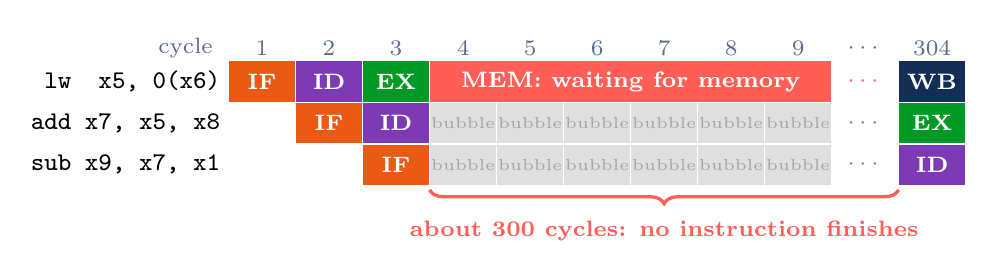
\begin{tikzpicture}[scale=1.15, every node/.append style={transform shape}]
      % cycle numbers (the last column is cycle 304)
      \node[font=\scriptsize, text=DeepBlue!70, anchor=east] at ({-0.5*\pw-0.05},{0.8*\ph}) {cycle};
      \foreach \c in {1,...,9}
        \node[font=\scriptsize, text=DeepBlue!70] at ({(\c-1)*\pw},{0.8*\ph}) {\c};
      \node[font=\scriptsize, text=DeepBlue!70] at ({9*\pw},{0.8*\ph}) {$\cdots$};
      \node[font=\scriptsize, text=DeepBlue!70] at ({10*\pw},{0.8*\ph}) {304};
      % lw: MEM takes about 300 cycles
      \plabel{0}{lw\ \ x5, 0(x6)}
      \prow{0}{1}{IF,ID,EX}
      \node[pcell, fill=MacRed, minimum width={6*\pw cm}] at ({5.5*\pw},0) {MEM: waiting for memory};
      \node[pcell, fill=none, draw=none, text=MacRed] at ({9*\pw},0) {$\cdots$};
      \prow{0}{11}{WB}
      % add: needs x5
      \plabel{1}{add x7, x5, x8}
      \prow{1}{2}{IF,ID,B,B,B,B,B,B}
      \node[pcell, fill=none, draw=none, text=gray] at ({9*\pw},{-\ph}) {$\cdots$};
      \prow{1}{11}{EX}
      % sub: stuck behind add
      \plabel{2}{sub x9, x7, x1}
      \prow{2}{3}{IF,B,B,B,B,B,B}
      \node[pcell, fill=none, draw=none, text=gray] at ({9*\pw},{-2*\ph}) {$\cdots$};
      \prow{2}{11}{ID}
      \draw[decorate, decoration={brace, amplitude=5pt, mirror}, very thick, MacRed]
        ({2.5*\pw},{-2.6*\ph}) -- ({9.5*\pw},{-2.6*\ph})
        node[midway, below=6pt, font=\scriptsize\bfseries, text=MacRed] {about 300 cycles: no instruction finishes};
    \end{tikzpicture}\\[0.15cm]
    \stagelegend
  \end{center}
  \vspace{0.1cm}
  \begin{beamercolorbox}[rounded=true,sep=0.1cm,wd=\textwidth]{block body}
    \centering\small The pipeline assumes that MEM takes \textbf{one} cycle. Main memory needs about \textbf{100 ns}
    $\approx$ \textbf{300 cycles} at 3 GHz:\\ \textbf{300 instructions} that could have finished, and none did.
  \end{beamercolorbox}
  \vfill
  \keymsg{A processor is only as fast as the data it gets. Today: \textbf{where the data comes from}.}
\end{frame}

% =====================================================================
\section{The memory wall}
% =====================================================================

\begin{frame}{How far away is the data?}
  \begin{beamercolorbox}[rounded=true,sep=0.12cm,wd=\textwidth]{block body}
    \centering\small Imagine that one clock cycle (about 0.3 ns at 3 GHz) takes \textbf{one second}.
  \end{beamercolorbox}
  \vspace{0.15cm}
  \begin{center}
    \footnotesize
    \renewcommand{\arraystretch}{1.18}
    \begin{tabular}{llrr}
      \toprule
      & \textbf{Where} & \textbf{Real time (approx.)} & \textbf{If 1 cycle = 1 second} \\
      \midrule
      \textcolor{cReg}{\rule{0.25cm}{0.25cm}}   & Register            & 0.3 ns          & 1 second \\
      \textcolor{cCache}{\rule{0.25cm}{0.25cm}} & L1 cache            & 1 ns            & a few seconds \\
      \textcolor{cCache}{\rule{0.25cm}{0.25cm}} & L2 cache            & 4 ns            & about 13 seconds \\
      \textcolor{cCache}{\rule{0.25cm}{0.25cm}} & L3 cache            & 15 ns           & about 1 minute \\
      \textcolor{cRAM}{\rule{0.25cm}{0.25cm}}   & Main memory (DRAM)  & 100 ns          & about \textbf{5 minutes} \\
      \textcolor{cDisk}{\rule{0.25cm}{0.25cm}}  & NVMe SSD            & 20--100 $\mu$s      & about \textbf{1--4 days} \\
      \textcolor{cDisk}{\rule{0.25cm}{0.25cm}}  & Hard disk (HDD)     & 5--10 ms        & about \textbf{6--12 months} \\
      \bottomrule
    \end{tabular}
  \end{center}
  \vfill
  \keymsg{From the CPU's point of view, RAM is a \textbf{coffee break} and a hard disk is a \textbf{year off}.}
\end{frame}

% ---------- small diagrams for the memory dilemma ----------
\newcommand{\diagSRAM}{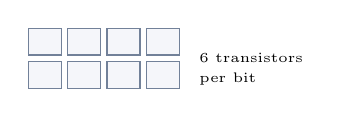
\begin{tikzpicture}
  \foreach \i in {0,...,3} \foreach \j in {0,1}
    \draw[DeepBlue!60, fill=LightGray] ({0.5*\i},{0.42*\j}) rectangle ++(0.42,0.34);
  \node[font=\tiny, anchor=west] at (2.05,0.38) {6 transistors};
  \node[font=\tiny, anchor=west] at (2.05,0.12) {per bit};
\end{tikzpicture}}
\newcommand{\diagDRAM}{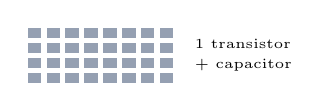
\begin{tikzpicture}
  \foreach \i in {0,...,7} \foreach \j in {0,...,3}
    \fill[DeepBlue!45] ({0.24*\i},{0.19*\j}) rectangle ++(0.17,0.13);
  \node[font=\tiny, anchor=west] at (2.0,0.5) {1 transistor};
  \node[font=\tiny, anchor=west] at (2.0,0.22) {+ capacitor};
\end{tikzpicture}}
\newcommand{\diagDiskSmall}{
\begin{tikzpicture}
  \draw[DeepBlue!60, thick, fill=LightGray] (0,0.35) circle (0.36);
  \draw[DeepBlue!60] (0,0.35) circle (0.22); \fill[DeepBlue!60] (0,0.35) circle (0.05);
  \draw[DeepBlue!60, fill=LightGray, rounded corners=2pt] (1.0,0.05) rectangle (1.75,0.65);
  \foreach \k in {0,1,2} \fill[DeepBlue!45] (1.1+0.22*\k,0.2) rectangle ++(0.14,0.3);
  \node[font=\tiny, anchor=west] at (1.95,0.35) {disk / flash};
\end{tikzpicture}}

\begin{frame}{No memory is both fast and cheap}
  \begin{columns}[T,onlytextwidth]
    \column{0.31\textwidth}
      \optcard{SRAM (used for caches)}{\diagSRAM}
        {answers in about 1 ns}
        {very expensive per bit: gigabytes would cost far too much}
    \column{0.31\textwidth}
      \optcard{DRAM (used for main memory)}{\diagDRAM}
        {cheap per bit: gigabytes are easy}
        {about 100 ns: the CPU waits hundreds of cycles}
    \column{0.31\textwidth}
      \optcard{Flash (used in SSDs)}{\diagDiskSmall}
        {very cheap per bit, keeps data without power}
        {20--100 $\mu$s: far too slow for every access}
  \end{columns}
  \vfill
  \keymsg{Fast memory is \textbf{expensive}, cheap memory is \textbf{slow}: no single technology gives us both.}
\end{frame}

\begin{frame}{The memory hierarchy}
  \begin{columns}[c,onlytextwidth]
    \column{0.58\textwidth}
      \centering
      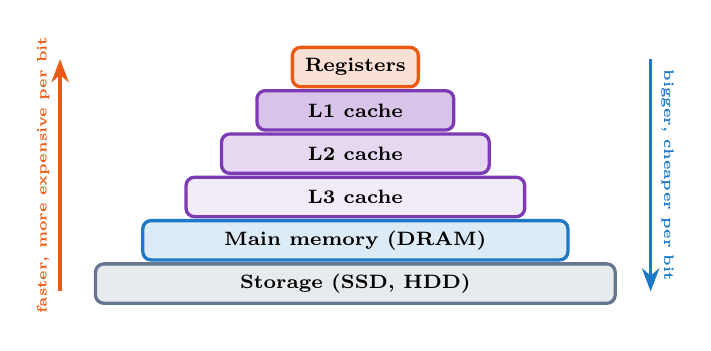
\begin{tikzpicture}[>=Stealth,
          lvl/.style={very thick, rounded corners=3pt, minimum height=0.5cm, font=\scriptsize\bfseries, inner sep=1pt}]
        \node[lvl, draw=cReg, fill=cReg!18, minimum width=1.6cm]   at (0,2.75) {Registers};
        \node[lvl, draw=cCache, fill=cCache!30, minimum width=2.5cm] at (0,2.2) {L1 cache};
        \node[lvl, draw=cCache, fill=cCache!20, minimum width=3.4cm] at (0,1.65) {L2 cache};
        \node[lvl, draw=cCache, fill=cCache!10, minimum width=4.3cm] at (0,1.1) {L3 cache};
        \node[lvl, draw=cRAM, fill=cRAM!15, minimum width=5.4cm]   at (0,0.55) {Main memory (DRAM)};
        \node[lvl, draw=cDisk, fill=cDisk!15, minimum width=6.6cm] at (0,0) {Storage (SSD, HDD)};
        \draw[->, very thick, AccentOrange] (-3.75,-0.1) -- (-3.75,2.85)
          node[midway, sloped, above, font=\tiny\bfseries] {faster, more expensive per bit};
        \draw[->, very thick, StorageBlue] (3.75,2.85) -- (3.75,-0.1)
          node[midway, sloped, above, font=\tiny\bfseries] {bigger, cheaper per bit};
      \end{tikzpicture}
    \column{0.4\textwidth}
      \stepbox{Near the CPU}{small and fast: registers and caches.}
      \stepbox{Far from the CPU}{big and slow: main memory and storage.}
  \end{columns}
  \vfill
  \keymsg{Goal: memory that \textbf{feels} as fast as the top and is as big as the bottom.}
\end{frame}

% =====================================================================
\section{Cache}
% =====================================================================

\begin{frame}{What is a cache? Hits and misses}
  \begin{columns}[c,onlytextwidth]
    \column{0.58\textwidth}
      \centering
      \begin{tikzpicture}[>=Stealth]
        \node[cpubox, minimum width=1.5cm, minimum height=1.2cm] (cpu) at (0,0) {\faMicrochip\\CPU};
        \node[cachebox, minimum width=1.4cm, minimum height=1.2cm] (c) at (2.6,0) {Cache\\[-1pt]\tiny small, fast};
        \node[rambox, minimum width=2.0cm, minimum height=1.9cm] (m) at (5.9,0) {Main memory\\[-1pt]\tiny big, slow};
        % hit
        \draw[okarr] ([yshift=0.35cm]cpu.east) -- ([yshift=0.35cm]c.west);
        \draw[okarr] ([yshift=0.15cm]c.west) -- ([yshift=0.15cm]cpu.east);
        \node[font=\scriptsize\bfseries, text=HitGreen, anchor=south] at (1.3,0.95) {hit: 1--4 cycles};
        % miss
        \draw[badarr] ([yshift=-0.2cm]cpu.east) -- ([yshift=-0.2cm]c.west);
        \draw[badarr] ([yshift=-0.2cm]c.east) -- ([yshift=-0.2cm]m.west);
        \draw[badarr] ([yshift=-0.45cm]m.west) -- ([yshift=-0.45cm]c.east);
        \draw[badarr] ([yshift=-0.45cm]c.west) -- ([yshift=-0.45cm]cpu.east);
        \node[font=\scriptsize\bfseries, text=MissRed, anchor=north] at (3.4,-1.15) {miss: hundreds of cycles};
      \end{tikzpicture}
    \column{0.4\textwidth}
      \defbox{\textbf{Cache}: a small, fast memory that keeps \textbf{copies} of recently used data from main memory.}
      \stepbox{Hit}{The data is in the cache: fast.}
      \stepbox{Miss}{The data is not there: fetch it from main memory, keep a copy, then use it.}
  \end{columns}
  \vfill
  \keymsg{The cache does not add new memory: it keeps \textbf{copies} close to the CPU. The program cannot see it.}
\end{frame}

\begin{frame}[fragile]{Why caching works: temporal locality}
  \defbox{\textbf{Temporal locality}: data used now will probably be used \textbf{again soon}.}
  \vspace{0.1cm}
  \begin{columns}[c,onlytextwidth]
    \column{0.4\textwidth}
\begin{lstlisting}[style=cc]
for (i = 0; @i@ < @n@; @i@++)
    @sum@ = @sum@ + a[i];
\end{lstlisting}
      \vspace{0.05cm}
      {\scriptsize \texttt{sum}, \texttt{i} and \texttt{n} are used in \textbf{every} iteration.\par}
    \column{0.56\textwidth}
      \centering
      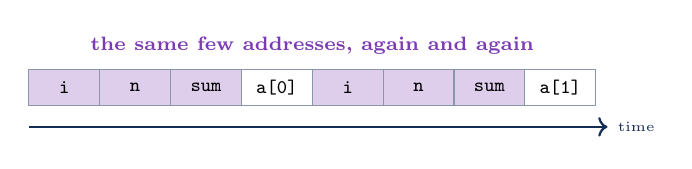
\begin{tikzpicture}[acc/.style={draw=DeepBlue!50, minimum width=0.9cm, minimum height=0.45cm,
          inner sep=0pt, font=\ttfamily\scriptsize}]
        \foreach \t/\f [count=\k from 0] in {i/1,n/1,sum/1,a[0]/0,i/1,n/1,sum/1,a[1]/0} {
          \ifnum\f=1 \def\fc{cCache!25}\else\def\fc{white}\fi
          \node[acc, fill=\fc] at ({0.9*\k},0) {\t};
        }
        \draw[->, thick, DeepBlue] (-0.45,-0.5) -- (6.9,-0.5) node[right, font=\tiny] {time};
        \node[font=\scriptsize\bfseries, text=cCache, anchor=south] at (3.15,0.3) {the same few addresses, again and again};
      \end{tikzpicture}
  \end{columns}
  \vspace{0.2cm}
  \stepbox{What the cache does}{It keeps \textbf{recently used} data close to the CPU, because it will probably be needed again.}
  \vfill
  \keymsg{Temporal locality: what was used \textbf{recently} is worth keeping close.}
\end{frame}

\begin{frame}[fragile]{Why caching works: spatial locality}
  \defbox{\textbf{Spatial locality}: data \textbf{next to} what we use now will probably be used soon.}
  \vspace{0.1cm}
  \begin{columns}[c,onlytextwidth]
    \column{0.4\textwidth}
\begin{lstlisting}[style=cc]
for (i = 0; i < n; i++)
    sum = sum + @a[i]@;
\end{lstlisting}
      \vspace{0.05cm}
      {\scriptsize \texttt{a[0]}, \texttt{a[1]}, \texttt{a[2]} \ldots\ are \textbf{neighbours} in memory.\par}
    \column{0.56\textwidth}
      \centering
      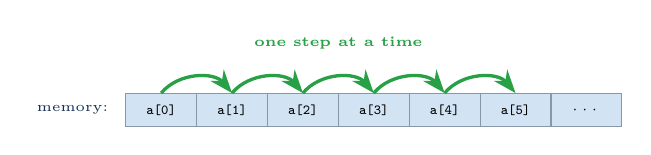
\begin{tikzpicture}[>=Stealth, cellm/.style={draw=DeepBlue!50, minimum width=0.9cm, minimum height=0.42cm,
          inner sep=0pt, font=\ttfamily\tiny, fill=StorageBlue!20}]
        \node[font=\tiny, text=DeepBlue, anchor=east] at (-0.55,0) {memory:};
        \foreach \t [count=\k from 0] in {a[0],a[1],a[2],a[3],a[4],a[5],$\cdots$}
          \node[cellm] (s\k) at ({0.9*\k},0) {\t};
        \foreach \k [evaluate=\k as \n using int(\k+1)] in {0,...,4}
          \draw[->, very thick, HitGreen] (s\k.north) to[bend left=50] (s\n.north);
        \node[font=\tiny\bfseries, text=HitGreen, anchor=south] at (2.25,0.65) {one step at a time};
      \end{tikzpicture}
  \end{columns}
  \vspace{0.2cm}
  \stepbox{What the cache does}{When it fetches data, it brings the \textbf{neighbours} too, because they will probably be needed soon.}
  \vfill
  \keymsg{Spatial locality: data \textbf{next to} what we use is worth fetching together.}
\end{frame}

% ---------- memory strip of the 2D array ----------
% #1 extra TikZ drawn on top
\newcommand{\arraystrip}[1]{%
  \begin{tikzpicture}[>=Stealth, cellm/.style={draw=DeepBlue!60, minimum width=1.2cm, minimum height=0.45cm,
      inner sep=0pt, font=\ttfamily\tiny, fill=StorageBlue!12}]
    \foreach \t [count=\k from 0] in {m[0][0],m[0][1],m[0][2],$\cdots$,m[0][99],m[1][0],m[1][1],$\cdots$,m[2][0]}
      \node[cellm] (c\k) at (1.2*\k,0) {\t};
    \node[font=\tiny, text=DeepBlue, anchor=east] at (-0.7,0) {memory:};
    #1
  \end{tikzpicture}}

\begin{frame}[fragile]{Exercise 1: find the locality}
  \begin{columns}[T,onlytextwidth]
    \column{0.47\textwidth}
      \taskhead{Task}{Two versions of the same program add up all elements of a 100 $\times$ 100 array
        \texttt{m}. In C, the array is stored \textbf{row by row}.}
      \footnotesize
      \begin{enumerate}\setlength{\itemsep}{3pt}
        \item Which variables show \textbf{temporal} locality?
        \item In memory, is \texttt{m[0][1]} next to \texttt{m[0][0]} or next to \texttt{m[1][0]}?
        \item Which version has better \textbf{spatial} locality? Why?
      \end{enumerate}
    \column{0.5\textwidth}
      {\scriptsize\textbf{Version A}: rows outside\par}
\begin{lstlisting}[style=cc]
for (i = 0; i < 100; i++)
    for (j = 0; j < 100; j++)
        total = total + m[i][j];
\end{lstlisting}
      {\scriptsize\textbf{Version B}: columns outside\par}
\begin{lstlisting}[style=cc]
for (j = 0; j < 100; j++)
    for (i = 0; i < 100; i++)
        total = total + m[i][j];
\end{lstlisting}
  \end{columns}
  \vfill
  \begin{center}
    \arraystrip{}
  \end{center}
\end{frame}

\begin{frame}{Solution: find the locality}
  \begin{center}
    \arraystrip{%
      \draw[->, very thick, HitGreen] (c0.north) to[bend left=50] (c1.north);
      \draw[->, very thick, HitGreen] (c1.north) to[bend left=50] (c2.north);
      \draw[->, very thick, HitGreen] (c2.north) to[bend left=50] (c3.north);
      \node[font=\scriptsize\bfseries, text=HitGreen, anchor=south] at (1.8,0.62) {A: one step at a time};
      \draw[->, very thick, MissRed] (c0.south) to[bend right=25] (c5.south);
      \draw[->, very thick, MissRed] (c5.south) to[bend right=35] (c8.south);
      \node[font=\scriptsize\bfseries, text=MissRed, anchor=north] at (6.0,-1.05) {B: jumps over 100 elements every time};
    }
  \end{center}
  \vspace{0.1cm}
  \begin{columns}[T,onlytextwidth]
    \column{0.31\textwidth}
      \stepbox{1. Temporal}{\texttt{total}, \texttt{i} and \texttt{j} are used in every iteration.}
    \column{0.31\textwidth}
      \stepbox{2. Layout}{\texttt{m[0][1]} comes right after \texttt{m[0][0]}: the array is stored row by row.}
    \column{0.31\textwidth}
      \stepbox{3. Spatial}{Version \textbf{A} reads neighbours one after another. Version B jumps.}
  \end{columns}
  \vfill
  \keymsg{Same result and the same work, but version B \textbf{jumps around} in memory. Next: measure what that costs.}
\end{frame}

\begin{frame}{Exercise 2: measure both versions}
  \taskhead{Task}{Put the two loops from Exercise 1 into a C program and measure how long each one takes.}
  \begin{columns}[T,onlytextwidth]
    \column{0.48\textwidth}
      \stepbox{How}{Use a \textbf{big} array: \texttt{static int m[4000][4000];} (64 MB), and fill it first.\\
        Measure each loop with \texttt{clock()} from \texttt{<time.h>}.\\
        Compile with optimisation: \texttt{gcc -O2}.}
    \column{0.48\textwidth}
      \footnotesize
      \begin{enumerate}\setlength{\itemsep}{4pt}
        \item Which version is faster? \textbf{How many times} faster?
        \item Why do we need a 4000 $\times$ 4000 array and not 100 $\times$ 100?
      \end{enumerate}
  \end{columns}
\end{frame}

\begin{frame}{Solution: measure both versions}
  \begin{columns}[c,onlytextwidth]
    \column{0.55\textwidth}
      \stepbox{1. Result}{On a test machine: A takes about \textbf{0.01 s}, B about \textbf{0.1 s}:
        B is about \textbf{10$\times$ slower}. Your numbers will differ, but B is clearly slower.}
      \stepbox{2. Why so big?}{100 $\times$ 100 ints = 40 KB: the whole array fits in the cache, so both versions
        hit and the difference disappears. 4000 $\times$ 4000 = 64 MB does not fit.}
    \column{0.4\textwidth}
      \centering
      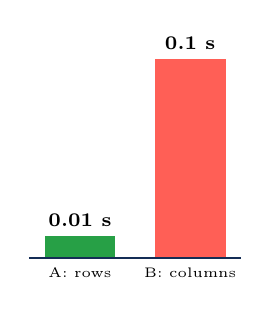
\begin{tikzpicture}
        \foreach \v/\l/\c [count=\k from 0] in {0.01/A: rows/HitGreen,0.1/B: columns/MissRed} {
          \fill[\c] ({1.4*\k},0) rectangle ++(0.9,{\v*25+0.03});
          \node[font=\scriptsize\bfseries, above] at ({1.4*\k+0.45},{\v*25+0.03}) {\v\ s};
          \node[font=\tiny, below] at ({1.4*\k+0.45},0) {\l};
        }
        \draw[thick, DeepBlue] (-0.2,0) -- (2.5,0);
      \end{tikzpicture}
  \end{columns}
  \vfill
  \keymsg{Same work, same result: only the \textbf{order} of the memory accesses changed.}
\end{frame}

\begin{frame}{The cache copies whole lines}
  \begin{center}
    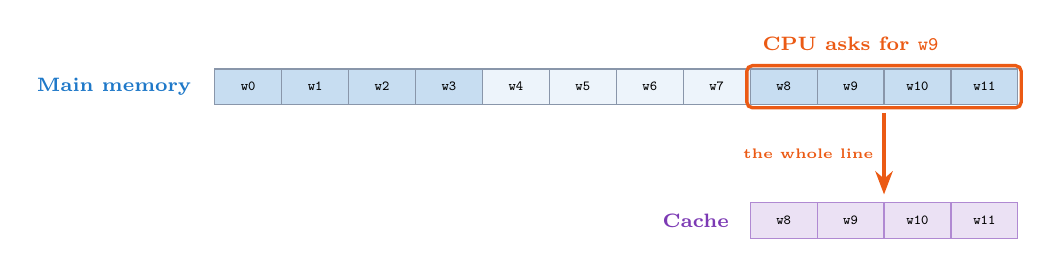
\begin{tikzpicture}[>=Stealth, w/.style={draw=DeepBlue!50, minimum width=0.85cm, minimum height=0.45cm,
        inner sep=0pt, font=\ttfamily\tiny}]
      \node[font=\scriptsize\bfseries, text=StorageBlue, anchor=east] at (-0.6,0) {Main memory};
      \foreach \k in {0,...,11} {
        \pgfmathtruncatemacro{\b}{int(\k/4)}
        \ifodd\b \def\fc{StorageBlue!8}\else\def\fc{StorageBlue!25}\fi
        \node[w, fill=\fc] (w\k) at (0.85*\k,0) {w\k};
      }
      \draw[AccentOrange, very thick, rounded corners=2pt] ([xshift=-1pt,yshift=1pt]w8.north west) rectangle ([xshift=1pt,yshift=-1pt]w11.south east);
      \node[font=\scriptsize\bfseries, text=AccentOrange, anchor=south] at ([yshift=3pt]w9.north) {CPU asks for \texttt{w9}};
      \foreach \k in {8,...,11}
        \node[w, fill=cCache!15, draw=cCache!60] (c\k) at ({0.85*\k},-1.7) {w\k};
      \node[font=\scriptsize\bfseries, text=cCache, anchor=east] at ([xshift=-4pt]c8.west) {Cache};
      \draw[->, very thick, AccentOrange] ($(w9.south)!0.5!(w10.south)+(0,-0.1)$) -- ($(c9.north)!0.5!(c10.north)+(0,0.1)$)
        node[midway, left, font=\tiny\bfseries] {the whole line};
    \end{tikzpicture}
  \end{center}
  \vspace{0.1cm}
  \defbox{\textbf{Cache line} (block): the unit copied between main memory and the cache.
    In today's processors: \textbf{64 bytes} = 16 words of 4 bytes. In our pictures: \textbf{4 words}, to keep them small.}
  \vfill
  \keymsg{One miss brings the whole line, so the next accesses to its neighbours are \textbf{hits}.}
\end{frame}

\begin{frame}{Which words come along?}
  \begin{center}
    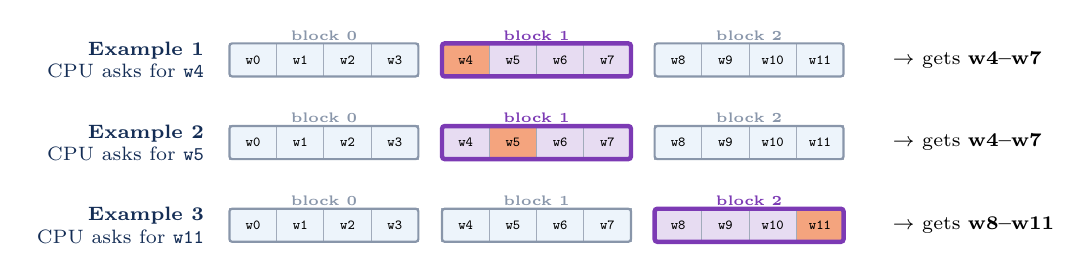
\begin{tikzpicture}[>=Stealth, w/.style={draw=DeepBlue!40, minimum width=0.6cm, minimum height=0.42cm,
        inner sep=0pt, font=\ttfamily\tiny}]
      \foreach \a/\b [count=\y from 1] in {4/1,5/1,11/2} {
        \pgfmathsetmacro{\yy}{-1.05*(\y-1)}
        \node[font=\scriptsize, text=DeepBlue, anchor=east, align=right] at (-0.5,\yy) {\textbf{Example \y}\\ CPU asks for \texttt{w\a}};
        \foreach \k in {0,...,11} {
          \pgfmathtruncatemacro{\kb}{int(\k/4)}
          \ifnum\kb=\b \def\fc{cCache!18}\else\def\fc{StorageBlue!8}\fi
          \ifnum\k=\a \def\fc{AccentOrange!55}\fi
          \node[w, fill=\fc] at ({0.6*\k+0.3*\kb},\yy) {w\k};
        }
        \foreach \bb in {0,1,2} {
          \ifnum\bb=\b \def\bc{cCache}\def\bw{1.6pt}\else\def\bc{DeepBlue!50}\def\bw{0.8pt}\fi
          \draw[\bc, line width=\bw, rounded corners=1pt] ({2.7*\bb-0.3},{\yy+0.21})
            rectangle ++(2.4,-0.42);
          \node[font=\tiny\bfseries, text=\bc, anchor=south, inner sep=1pt] at ({2.7*\bb+0.9},{\yy+0.21}) {block \bb};
        }
        \pgfmathtruncatemacro{\f}{4*\b}\pgfmathtruncatemacro{\l}{4*\b+3}
        \node[font=\scriptsize, anchor=west] at (8.0,\yy) {$\rightarrow$ gets \textbf{w\f--w\l}};
      }
    \end{tikzpicture}
  \end{center}
  \vspace{0.1cm}
  \stepbox{Fixed blocks}{Memory is split into fixed blocks of 4 words, and every word belongs to exactly \textbf{one} block.
    The whole block is copied, so the neighbours can be on the \textbf{right}, on the \textbf{left} or on \textbf{both} sides.}
  \vfill
  \keymsg{The block boundaries \textbf{never move}: the requested word can be at the start, in the middle or at the end.}
\end{frame}

% memory drawn as a grid with one column per cache line
% #1 extra TikZ; nodes: g<block>, line<c>
\newcommand{\dmgrid}[1]{%
  \begin{tikzpicture}[>=Stealth, gb/.style={minimum width=0.95cm, minimum height=0.42cm, inner sep=0pt,
      font=\ttfamily\scriptsize}]
    \node[font=\scriptsize\bfseries, text=StorageBlue] at (1.5,0.55) {Main memory (blocks)};
    \foreach \r in {0,...,3} \foreach \c in {0,...,3} {
      \pgfmathtruncatemacro{\bn}{4*\r+\c}
      \node[gb, draw=StorageBlue!60, fill=StorageBlue!12] (g\bn) at (\c,{-0.45*\r}) {\bn};
    }
    \foreach \c in {0,...,3} {
      \node[gb, draw=cCache, very thick, fill=cCache!15, font=\scriptsize\bfseries] (line\c) at (\c,-2.55) {line \c};
      \draw[->, thick, DeepBlue!50] (\c,-1.6) -- (line\c.north);
    }
    \node[font=\scriptsize\bfseries, text=cCache, anchor=east] at (-0.6,-2.55) {Cache};
    #1
  \end{tikzpicture}}

\begin{frame}{The cache is small}
  \begin{center}
    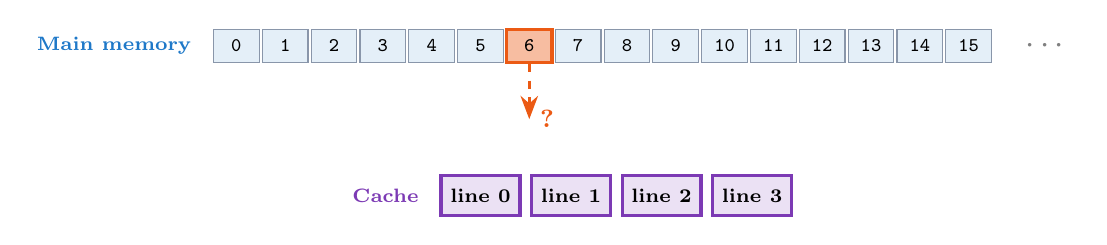
\begin{tikzpicture}[>=Stealth, mb/.style={draw=DeepBlue!50, fill=StorageBlue!12, minimum width=0.58cm,
        minimum height=0.42cm, inner sep=0pt, font=\ttfamily\scriptsize}]
      \node[font=\scriptsize\bfseries, text=StorageBlue, anchor=east] at (-0.45,0) {Main memory};
      \foreach \k in {0,...,15}
        \node[mb] (m\k) at ({0.62*\k},0) {\k};
      \node[mb, fill=AccentOrange!40, draw=AccentOrange, very thick] (m6) at ({0.62*6},0) {6};
      \node[font=\large, text=gray] at (10.3,0) {$\cdots$};
      \foreach \c in {0,...,3}
        \node[draw=cCache, very thick, fill=cCache!15, minimum width=1.0cm, minimum height=0.5cm, inner sep=0pt,
          font=\scriptsize\bfseries] (l\c) at ({3.1+1.15*\c},-1.9) {line \c};
      \node[font=\scriptsize\bfseries, text=cCache, anchor=east] at ([xshift=-4pt]l0.west) {Cache};
      \draw[->, very thick, AccentOrange, dashed] (m6.south) -- ++(0,-0.7) node[right, font=\small\bfseries, text=AccentOrange] {?};
    \end{tikzpicture}
  \end{center}
  \vspace{0.15cm}
  \stepbox{The problem}{Main memory has millions of blocks, the cache only a few lines (here: 4).
    Block 6 has just been read: \textbf{which line} should keep it?}
  \vfill
  \keymsg{We need a simple, fast rule: \textbf{block number $\rightarrow$ line}.}
\end{frame}

\begin{frame}{Direct mapping: the column is the line}
  \begin{columns}[c,onlytextwidth]
    \column{0.45\textwidth}
      \centering
      \dmgrid{%
        \node[minimum width=0.95cm, minimum height=0.42cm, draw=AccentOrange, fill=AccentOrange!35, line width=1.8pt,
          font=\ttfamily\scriptsize] at (g6) {6};
        \draw[->, very thick, AccentOrange] (2,-1.6) -- (line2.north);
        \node[minimum width=0.95cm, minimum height=0.42cm, draw=AccentOrange, line width=1.8pt] at (line2) {};}
    \column{0.52\textwidth}
      \stepbox{Draw memory with 4 columns}{one column for each line of the cache. Every block goes to the line
        \textbf{under its column}.}
      \stepbox{The rule}{line = block number \textbf{mod} 4\\ block 6 $\rightarrow$ 6 mod 4 = 2 $\rightarrow$ line 2}
      \stepbox{Sharing}{Blocks 2, 6, 10 and 14 all use line 2: only one of them can be in the cache at a time.}
  \end{columns}
  \vfill
  \keymsg{Direct-mapped cache: every block has exactly \textbf{one} line, so there is only one place to look.}
  \simfoot{\simlink{cache}}
\end{frame}

\begin{frame}{How does the cache know which block it holds?}
  \begin{columns}[c,onlytextwidth]
    \column{0.47\textwidth}
      \centering
      \dmgrid{%
        \foreach \r in {0,...,3}
          \node[font=\scriptsize\bfseries, text=DeepBlue, anchor=east] at (-0.55,{-0.45*\r}) {row \r};
        \node[minimum width=0.95cm, minimum height=0.42cm, draw=AccentOrange, fill=AccentOrange!35, line width=1.8pt,
          font=\ttfamily\scriptsize] at (g6) {6};
        \foreach \c/\t in {0/0,1/--,2/1,3/0}
          \node[minimum width=0.95cm, minimum height=0.42cm, inner sep=0pt, draw=cCache, fill=white,
            font=\ttfamily\scriptsize] (tag\c) at (\c,-3.0) {\t};
        \node[draw=AccentOrange, line width=1.8pt, minimum width=0.95cm, minimum height=0.42cm] at (tag2) {};
        \node[font=\scriptsize\bfseries, text=cCache, anchor=east] at (-0.6,-3.0) {Tag};}
    \column{0.5\textwidth}
      \stepbox{The problem}{The CPU does not know whether line 2 holds block 2, 6, 10 or 14.
        The line must be \textbf{marked} somehow.}
      \stepbox{The tag}{Next to the data, every line stores a tag: the \textbf{row} of its block.\\[0.05cm]
        $\text{tag} = \left\lfloor \dfrac{\text{block number}}{4} \right\rfloor$ \qquad
        block 6: $\left\lfloor \frac{6}{4} \right\rfloor = 1$}
      \stepbox{Empty lines}{A \textbf{valid bit} marks whether a line holds a block at all (line 1: nothing yet).}
  \end{columns}
  \vfill
  \keymsg{Hit: the line of the block is valid and holds the \textbf{same tag}.}
\end{frame}

\begin{frame}{Exercise 3: line and tag}
  \taskhead{Task}{A direct-mapped cache with \textbf{4 lines}, as in the pictures: line = block \textbf{mod} 4,
    $\text{tag} = \left\lfloor \text{block} / 4 \right\rfloor$.}
  \begin{columns}[T,onlytextwidth]
    \column{0.44\textwidth}
      \footnotesize
      \textbf{1.} For each block, give its line and its tag:\\[0.1cm]
      \centering
      \renewcommand{\arraystretch}{1.2}
      \begin{tabular}{ccc}
        \toprule
        \textbf{Block} & \textbf{Line} & \textbf{Tag} \\
        \midrule
        5 & \ldots & \ldots \\ 12 & \ldots & \ldots \\ 7 & \ldots & \ldots \\ 9 & \ldots & \ldots \\
        \bottomrule
      \end{tabular}
    \column{0.52\textwidth}
      \footnotesize
      \textbf{2.} The cache now holds:\\[0.1cm]
      \centering
      \renewcommand{\arraystretch}{1.2}
      \begin{tabular}{ccccc}
        \toprule
        \textbf{Line} & 0 & 1 & 2 & 3 \\
        \midrule
        \textbf{Tag} & 3 & 2 & empty & 1 \\
        \bottomrule
      \end{tabular}\\[0.15cm]
      \raggedright
      Is each access a \textbf{hit} or a \textbf{miss}? Block \textbf{9}, block \textbf{13}, block \textbf{6}, block \textbf{7}.
  \end{columns}
  \simfoot{\simlink{cache}}
\end{frame}

\begin{frame}{Solution: line and tag}
  \begin{columns}[T,onlytextwidth]
    \column{0.4\textwidth}
      \centering\footnotesize
      \textbf{1. Line and tag}\\[0.1cm]
      \renewcommand{\arraystretch}{1.2}
      \begin{tabular}{ccc}
        \toprule
        \textbf{Block} & \textbf{Line} (mod 4) & \textbf{Tag} ($\lfloor / 4 \rfloor$) \\
        \midrule
        5 & 1 & 1 \\ 12 & 0 & 3 \\ 7 & 3 & 1 \\ 9 & 1 & 2 \\
        \bottomrule
      \end{tabular}
    \column{0.56\textwidth}
      \centering\footnotesize
      \textbf{2. Hit or miss?}\\[0.1cm]
      \renewcommand{\arraystretch}{1.2}
      \begin{tabular}{cccl}
        \toprule
        \textbf{Block} & \textbf{Line} & \textbf{Tag} & \textbf{Result} \\
        \midrule
        9 & 1 & 2 & \textcolor{HitGreen}{\textbf{hit}}: line 1 holds tag 2 \\
        13 & 1 & 3 & \textcolor{MissRed}{\textbf{miss}}: line 1 holds tag 2 (block 9) \\
        6 & 2 & 1 & \textcolor{MissRed}{\textbf{miss}}: line 2 is empty \\
        7 & 3 & 1 & \textcolor{HitGreen}{\textbf{hit}}: line 3 holds tag 1 \\
        \bottomrule
      \end{tabular}
  \end{columns}
  \vfill
  \keymsg{Block 13 misses although line 1 is full: the line holds a \textbf{different} block with the same line number.}
\end{frame}

\begin{frame}{Set-associative caches: two places for every block}
  \begin{columns}[c,onlytextwidth]
    \column{0.4\textwidth}
      \centering
      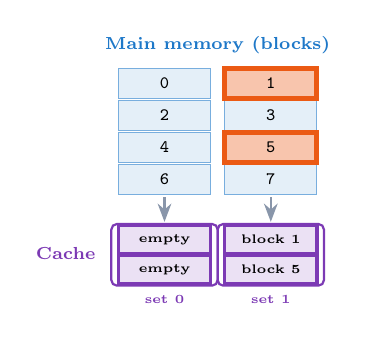
\begin{tikzpicture}[>=Stealth, scale=0.9, every node/.append style={transform shape}, gb/.style={minimum width=1.3cm, minimum height=0.42cm, inner sep=0pt,
          font=\ttfamily\scriptsize}]
        \colorlet{sc0}{cCache}\colorlet{sc1}{cCache}
        \node[font=\scriptsize\bfseries, text=StorageBlue] at (0.75,0.55) {Main memory (blocks)};
        \foreach \r in {0,...,3} \foreach \c in {0,1} {
          \pgfmathtruncatemacro{\bn}{2*\r+\c}
          \node[gb, draw=StorageBlue!60, fill=StorageBlue!12] (g\bn) at ({1.5*\c},{-0.45*\r}) {\bn};
        }
        \foreach \b in {1,5} \node[gb, draw=AccentOrange, fill=AccentOrange!35, line width=1.8pt] at (g\b) {\b};
        \foreach \c/\ta/\tb in {0/empty/empty,1/block 1/block 5} {
          \draw[->, thick, DeepBlue!50] ({1.5*\c},-1.6) -- ({1.5*\c},-1.95);
          \node[draw=sc\c, very thick, fill=sc\c!15, minimum width=1.3cm, minimum height=0.4cm, inner sep=0pt,
            font=\tiny\bfseries] at ({1.5*\c},-2.2) {\ta};
          \node[draw=sc\c, very thick, fill=sc\c!15, minimum width=1.3cm, minimum height=0.4cm, inner sep=0pt,
            font=\tiny\bfseries] at ({1.5*\c},-2.62) {\tb};
          \draw[sc\c, thick, rounded corners=2pt] ({1.5*\c-0.75},-1.98) rectangle ({1.5*\c+0.75},-2.85);
          \node[font=\tiny\bfseries, text=sc\c, anchor=north] at ({1.5*\c},-2.87) {set \c};
        }
        \node[font=\scriptsize\bfseries, text=cCache, anchor=east] at (-0.85,-2.4) {Cache};
      \end{tikzpicture}
    \column{0.57\textwidth}
      \centering
      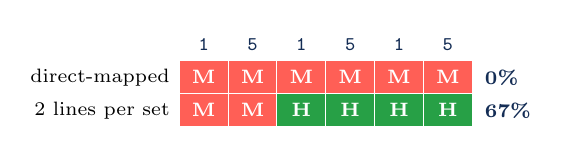
\begin{tikzpicture}
        \hmhead{0}{1,5,1,5,1,5}
        \hmlabel{1}{direct-mapped} \hmrow{1}{M,M,M,M,M,M} \hmresult{1}{6}{0\%}
        \hmlabel{2}{2 lines per set} \hmrow{2}{M,M,H,H,H,H} \hmresult{2}{6}{67\%}
      \end{tikzpicture}\\[0.1cm]
      \raggedright
      \stepbox{The problem}{In a direct-mapped cache, blocks 1 and 5 both need line 1 and keep throwing each other out.}
      \stepbox{The fix}{Group the lines into \textbf{sets}: set = block \textbf{mod} 2. A block may use any line of its set,
        so 1 and 5 fit together. When a set is full, the \textbf{least recently used} line goes out (LRU).}
  \end{columns}
  \vfill
  \keymsg{Real L1, L2 and L3 caches are \textbf{set-associative}, typically with 8 to 16 lines per set.}
\end{frame}

\begin{frame}{Exercise 4: hits and misses by hand}
  \taskhead{Task}{A cache with \textbf{4 lines}, 1 block per line, initially empty.
    The program reads blocks \textbf{0, 4, 1, 0, 4, 1}. For every access write \textbf{H} (hit) or \textbf{M} (miss).}
  \begin{columns}[T,onlytextwidth]
    \column{0.55\textwidth}
      \centering
      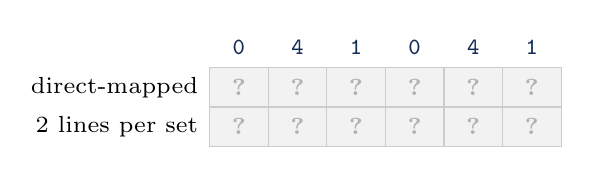
\begin{tikzpicture}[scale=1.2, every node/.append style={transform shape}]
        \hmhead{0}{0,4,1,0,4,1}
        \hmlabel{1}{direct-mapped} \hmrow{1}{Q,Q,Q,Q,Q,Q}
        \hmlabel{2}{2 lines per set} \hmrow{2}{Q,Q,Q,Q,Q,Q}
      \end{tikzpicture}
    \column{0.42\textwidth}
      \footnotesize
      \begin{enumerate}\setlength{\itemsep}{3pt}
        \item \textbf{Direct-mapped}: line = block \textbf{mod} 4.
        \item \textbf{2 lines per set}: the same 4 lines, 2 sets, set = block \textbf{mod} 2.
        \item What is the \textbf{hit rate} of each?
      \end{enumerate}
  \end{columns}
  \simfoot{\simlink{cache}}
\end{frame}

\begin{frame}{Solution: hits and misses by hand}
  \begin{columns}[c,onlytextwidth]
    \column{0.55\textwidth}
      \centering
      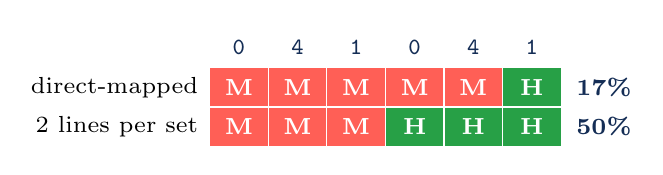
\begin{tikzpicture}[scale=1.2, every node/.append style={transform shape}]
        \hmhead{0}{0,4,1,0,4,1}
        \hmlabel{1}{direct-mapped} \hmrow{1}{M,M,M,M,M,H} \hmresult{1}{6}{17\%}
        \hmlabel{2}{2 lines per set} \hmrow{2}{M,M,M,H,H,H} \hmresult{2}{6}{50\%}
      \end{tikzpicture}
    \column{0.42\textwidth}
      \scriptsize
      \textbf{Direct-mapped}: 0 and 4 both use line 0 and throw each other out. Block 1 has line 1 for itself,
      so its second access hits.\\[0.1cm]
      \textbf{2 lines per set}: 0 and 4 share set 0, which has two lines: after the first reads, everything hits.
  \end{columns}
  \vspace{0.4cm}
  \begin{columns}[T,onlytextwidth]
    \column{0.31\textwidth}
      \stepbox{Compulsory miss}{The first access to a block always misses.}
    \column{0.31\textwidth}
      \stepbox{Conflict miss}{Another block that uses the same line (or set) threw it out.}
    \column{0.31\textwidth}
      \stepbox{Capacity miss}{The data simply does not fit in the cache.}
  \end{columns}
  \vfill
  \keymsg{More places per block removes \textbf{conflict} misses, but not compulsory or capacity misses.}
\end{frame}

\begin{frame}{How good is a cache? Hit rate, miss penalty, AMAT}
  \begin{columns}[T,onlytextwidth]
    \column{0.31\textwidth}
      \defbox{\textbf{Hit rate}: the fraction of accesses that hit.\\ \textbf{Miss rate} = 1 $-$ hit rate.}
    \column{0.31\textwidth}
      \defbox{\textbf{Hit time}: how long a hit takes.\\ \phantom{x}}
    \column{0.31\textwidth}
      \defbox{\textbf{Miss penalty}: the extra time to bring the line from the next level.}
  \end{columns}
  \vspace{0.15cm}
  \begin{beamercolorbox}[rounded=true,sep=0.14cm,wd=\textwidth]{block body}
    \centering
    \textbf{Average Memory Access Time}\\[0.05cm]
    $\displaystyle \text{AMAT} = \text{hit time} + \text{miss rate} \times \text{miss penalty}$
  \end{beamercolorbox}
  \vfill
  \keymsg{Misses are rare, but each one costs many cycles: AMAT combines both.}
\end{frame}

\begin{frame}{Exercise 5: AMAT}
  \begin{columns}[T,onlytextwidth]
    \column{0.48\textwidth}
      \taskhead{Part A}{An L1 cache with:}
      \footnotesize
      \begin{itemize}\setlength{\itemsep}{2pt}
        \item hit time = 1 cycle
        \item miss rate = 4\%, miss penalty = 10 cycles
      \end{itemize}
      \vspace{0.1cm}
      \textbf{1.} What is the AMAT?\\
      \textbf{2.} A program makes 1\,000\,000 memory accesses. How many cycles do they take? And with no misses at all?
    \column{0.48\textwidth}
      \taskhead{Part B: which cache is better?}{Two designs of an L1 cache:}
      \footnotesize
      \begin{itemize}\setlength{\itemsep}{2pt}
        \item \textbf{Design A}: hit time 1 cycle, miss rate 8\%, miss penalty 25 cycles
        \item \textbf{Design B}: hit time 2 cycles, miss rate 3\%, miss penalty 25 cycles
      \end{itemize}
      \vspace{0.1cm}
      Compute the AMAT of each. Which one is better, and why?
  \end{columns}
  \vfill
  \begin{beamercolorbox}[rounded=true,sep=0.1cm,wd=\textwidth]{block body}
    \scriptsize\textbf{Part C (if you finish early):} L1 hit time 1 cycle, miss rate 5\%.
    L2 hit time 10 cycles, and 20\% of the L1 misses also miss in L2. Main memory: 200 cycles.
    What is the AMAT with the L2 cache? And without it?
  \end{beamercolorbox}
\end{frame}

\begin{frame}{Solution: AMAT}
  \begin{columns}[T,onlytextwidth]
    \column{0.31\textwidth}
      \stepbox{Part A}{AMAT = 1 + 0.04 $\times$ 10 = \textbf{1.4 cycles}\\[0.1cm]
        1\,000\,000 $\times$ 1.4 = \textbf{1\,400\,000 cycles}; with no misses: 1\,000\,000\\[0.1cm]
        A miss rate of only 4\% makes memory access \textbf{40\% slower}.}
    \column{0.31\textwidth}
      \stepbox{Part B}{A: 1 + 0.08 $\times$ 25 = \textbf{3.0 cycles}\\[0.1cm]
        B: 2 + 0.03 $\times$ 25 = \textbf{2.75 cycles}\\[0.1cm]
        \textbf{B is better}, even though each of its hits is twice as slow.}
    \column{0.31\textwidth}
      \stepbox{Part C}{With L2:\\ 1 + 0.05 $\times$ (10 + 0.2 $\times$ 200) = \textbf{3.5 cycles}\\[0.1cm]
        Without L2:\\ 1 + 0.05 $\times$ 200 = \textbf{11 cycles}}
  \end{columns}
  \vfill
  \keymsg{Misses are rare but \textbf{expensive}, so a lower miss rate often beats a faster hit.}
\end{frame}

\begin{frame}[fragile]{Exercise 6: see the cache in Ripes}
  \begin{columns}[T,onlytextwidth]
    \column{0.44\textwidth}
\begin{lstlisting}[style=rv]
.data
arr:  .zero 1024     # 256 words
.text
      li   x9, 2     # two passes
pass: la   x5, arr   # start of arr
      li   x6, 32    # N: reads per pass
loop: lw   x7, 0(x5)
      add  x10, x10, x7
      addi x5, x5, 4 # STRIDE in bytes
      addi x6, x6, -1
      bnez x6, loop
      addi x9, x9, -1
      bnez x9, pass
\end{lstlisting}
    \column{0.53\textwidth}
      \taskhead{Ripes task}{Open the \textbf{Cache} tab. Data cache: direct-mapped, \textbf{16 lines},
        \textbf{4 words per line} (256 bytes). \textbf{Predict first}, then run and read the hit rate.}
      \centering\scriptsize
      \renewcommand{\arraystretch}{1.2}
      \begin{tabular}{ccccc}
        \toprule
        Run & STRIDE & N & Predicted & Ripes \\
        \midrule
        1 & 4  & 32  & \ldots & \ldots \\
        2 & 16 & 32  & \ldots & \ldots \\
        3 & 16 & 16  & \ldots & \ldots \\
        4 & 4  & 128 & \ldots & \ldots \\
        \bottomrule
      \end{tabular}\\[0.15cm]
      \raggedright
      Which run shows a \textbf{capacity} problem? Which one shows pure \textbf{spatial locality}?
  \end{columns}
\end{frame}

\begin{frame}{Solution: see the cache in Ripes}
  \begin{center}
    \scriptsize
    \renewcommand{\arraystretch}{1.2}
    \begin{tabular}{lcccl}
      \toprule
      \textbf{Run} & \textbf{Reads} & \textbf{Misses} & \textbf{Hit rate} & \textbf{Why} \\
      \midrule
      1: stride 4, N 32   & 64  & 8  & \textbf{87.5\%} & 1 miss per 4 words; 128 B fit, so pass 2 only hits \\
      2: stride 16, N 32  & 64  & 64 & \textbf{0\%}    & every read is a new line; 32 lines $>$ 16 lines, so pass 2 misses too \\
      3: stride 16, N 16  & 32  & 16 & \textbf{50\%}   & pass 1 always misses, but 16 lines fit, so pass 2 hits \\
      4: stride 4, N 128  & 256 & 64 & \textbf{75\%}   & 512 B $>$ 256 B: nothing is left from pass 1 \\
      \bottomrule
    \end{tabular}
  \end{center}
  \vspace{0.05cm}
  \begin{columns}[T,onlytextwidth]
    \column{0.48\textwidth}
      \stepbox{Runs 1 and 2}{The same number of reads, but spatial locality is lost: the hit rate falls from 87.5\% to 0\%.}
    \column{0.48\textwidth}
      \stepbox{Runs 1 and 4}{The same stride, but the data stopped fitting in the cache: \textbf{capacity} misses. Run 4 shows \textbf{pure spatial locality}: nothing is reused, every hit is a neighbour in the same line.}
  \end{columns}
  \vfill
  \keymsg{The same instructions with a different memory pattern: the hit rate can go from \textbf{87.5\% to 0\%}.}
\end{frame}

\begin{frame}{Many levels of cache}
  \begin{columns}[c,onlytextwidth]
    \column{0.55\textwidth}
      \centering
      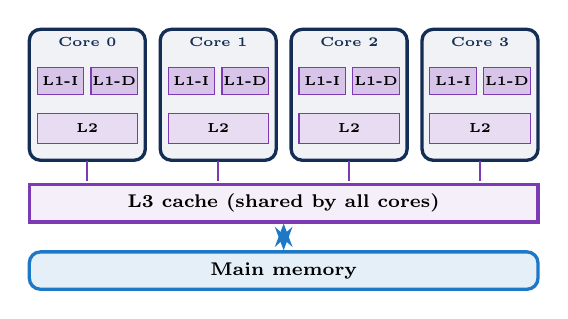
\begin{tikzpicture}[>=Stealth, scale=0.95, every node/.append style={transform shape}]
        \foreach \c in {0,...,3} {
          \node[draw=DeepBlue, very thick, rounded corners=4pt, fill=DeepBlue!6, minimum width=1.55cm,
            minimum height=1.75cm] (core\c) at ({1.75*\c},0) {};
          \node[font=\tiny\bfseries, text=DeepBlue, anchor=north] at (core\c.north) {Core \c};
          \node[draw=cCache, fill=cCache!30, minimum width=0.62cm, minimum height=0.36cm, inner sep=0pt,
            font=\tiny\bfseries] at ({1.75*\c-0.36},0.18) {L1-I};
          \node[draw=cCache, fill=cCache!30, minimum width=0.62cm, minimum height=0.36cm, inner sep=0pt,
            font=\tiny\bfseries] at ({1.75*\c+0.36},0.18) {L1-D};
          \node[draw=cCache, fill=cCache!18, minimum width=1.34cm, minimum height=0.4cm, inner sep=0pt,
            font=\tiny\bfseries] at ({1.75*\c},-0.45) {L2};
          \draw[thick, cCache] ({1.75*\c},-0.88) -- ({1.75*\c},-1.15);
        }
        \node[draw=cCache, very thick, fill=cCache!8, minimum width=6.8cm, minimum height=0.5cm,
          font=\scriptsize\bfseries] (l3) at (2.625,-1.45) {L3 cache (shared by all cores)};
        \node[rambox, minimum width=6.8cm, minimum height=0.5cm] (ram) at (2.625,-2.35) {Main memory};
        \draw[<->, very thick, cRAM] (l3.south) -- (ram.north);
      \end{tikzpicture}
    \column{0.43\textwidth}
      \stepbox{L1}{tens of KB, about 4 cycles, \textbf{split} into instructions (I) and data (D)}
      \stepbox{L2}{hundreds of KB to a few MB, about 12 cycles, one per core}
      \stepbox{L3}{tens of MB, about 40 cycles, \textbf{shared} by all cores. The same SRAM as L1: \textbf{bigger is slower}.}
  \end{columns}
  \vspace{0.1cm}
  \begin{beamercolorbox}[rounded=true,sep=0.08cm,wd=\textwidth]{block body}
    \scriptsize Split L1 = separate paths for instructions and data = the \textbf{modified Harvard} architecture.
    It also removes the structural hazard between IF and MEM in the pipeline.
  \end{beamercolorbox}
  \vfill
  \keymsg{Each level catches most misses of the level above, so only \textbf{few} accesses go all the way to main memory.}
\end{frame}

% Values checked against the manufacturers' published specifications (Intel Raptor Lake / Apple M3).
% Please verify again before class: vendors rarely publish every cache detail.
\begin{frame}{Real-world reveal: two laptops, one idea}
  \begin{center}
    \footnotesize
    \renewcommand{\arraystretch}{1.25}
    \begin{tabular}{lll}
      \toprule
      & \textbf{Intel Core i9-14900HX} & \textbf{Apple M3} \\
      \midrule
      Instruction set & x86-64 (CISC outside) & ARM64 (RISC) \\
      Cores & 8 performance + 16 efficiency & 4 performance + 4 efficiency \\
      L1 per performance core & 32 KB (I) + 48 KB (D) & 192 KB (I) + 128 KB (D) \\
      L2 & 2 MB per performance core & 16 MB shared by the performance cores \\
      Last level & 36 MB L3, shared by all cores & system level cache, shared \\
      Main memory & separate DDR5 modules & unified memory in the chip package \\
      \bottomrule
    \end{tabular}
  \end{center}
  \vfill
  \keymsg{Two different instruction sets, the \textbf{same} idea: a small split L1, a bigger L2, a big shared last level.}
\end{frame}

\begin{frame}{Task: what cache does your laptop have?}
  \begin{columns}[T,onlytextwidth]
    \column{0.31\textwidth}
      \begin{beamercolorbox}[rounded=true,sep=0.14cm,wd=\linewidth]{block body}
        \centering{\Huge\textcolor{DeepBlue}{\faWindows}}\\[0.12cm]
        \small\textbf{Windows}\\[0.05cm]
        \footnotesize Task Manager $\rightarrow$ Performance $\rightarrow$ CPU\\
        (L1, L2, L3 at the bottom right)
      \end{beamercolorbox}
    \column{0.31\textwidth}
      \begin{beamercolorbox}[rounded=true,sep=0.14cm,wd=\linewidth]{block body}
        \centering{\Huge\textcolor{DeepBlue}{\faLinux}}\\[0.12cm]
        \small\textbf{Linux}\\[0.05cm]
        \footnotesize\texttt{lscpu | grep -i cache}\\ \phantom{x}
      \end{beamercolorbox}
    \column{0.31\textwidth}
      \begin{beamercolorbox}[rounded=true,sep=0.14cm,wd=\linewidth]{block body}
        \centering{\Huge\textcolor{DeepBlue}{\faApple}}\\[0.12cm]
        \small\textbf{macOS}\\[0.05cm]
        \footnotesize\texttt{sysctl -a | grep cachesize}\\ \phantom{x}
      \end{beamercolorbox}
  \end{columns}
  \vspace{0.2cm}
  \taskhead{Task}{Write down the sizes of your L1, L2 and L3 caches. Is your L1 split into instructions and data?}
  \vfill
  \keymsg{Software can \textbf{read} the cache sizes, but it cannot choose what is inside: the hardware decides.}
\end{frame}

\begin{frame}[fragile]{Solution: what cache does your laptop have?}
  \begin{columns}[c,onlytextwidth]
    \column{0.5\textwidth}
      {\scriptsize Example: Intel Core i9-14900HX, Linux\par}
\begin{lstlisting}[style=asm]
$ lscpu | grep -i cache
L1d cache:  896 KiB (24 instances)
L1i cache:  1.3 MiB (24 instances)
L2 cache:   32 MiB (12 instances)
L3 cache:   36 MiB (1 instance)
\end{lstlisting}
    \column{0.46\textwidth}
      \stepbox{Split L1?}{Yes: \textbf{L1d} (data) and \textbf{L1i} (instructions) are separate caches.}
      \stepbox{Totals}{The numbers add up all cores. L3 has \textbf{1 instance}: one L3 shared by all cores.}
  \end{columns}
  \vfill
  \keymsg{The same structure everywhere: a split L1, a bigger L2 and one big \textbf{shared} L3.}
\end{frame}

% =====================================================================
\section{Summary}
% =====================================================================

\begin{frame}{What we saw today}
  \begin{center}
    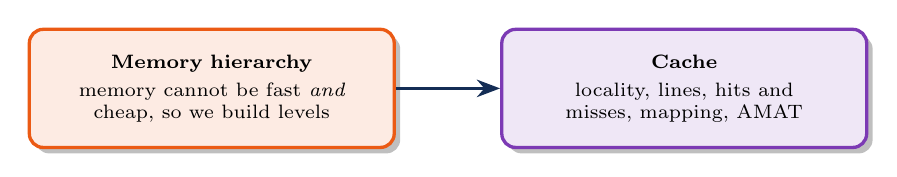
\begin{tikzpicture}[>=Stealth,
        sbox/.style={very thick, rounded corners=5pt, minimum width=4.6cm, minimum height=1.5cm,
          align=center, font=\scriptsize, text width=4.4cm, drop shadow}]
      \node[sbox, draw=AccentOrange, fill=AccentOrange!12] (a) at (0,0)
        {\textbf{Memory hierarchy}\\[2pt] memory cannot be fast \emph{and} cheap, so we build levels};
      \node[sbox, draw=ProgramPurple, fill=ProgramPurple!12] (b) at (6,0)
        {\textbf{Cache}\\[2pt] locality, lines, hits and misses, mapping, AMAT};
      \draw[->, very thick, DeepBlue] (a) -- (b);
    \end{tikzpicture}
  \end{center}
  \vfill
  \keymsg{A fast CPU is only as fast as the data it gets: the cache keeps that data \textbf{close}.}
\end{frame}

\begin{frame}{Check yourself}
  \footnotesize
  \begin{enumerate}\setlength{\itemsep}{6pt}
    \item Why can a better cache help more than a higher clock speed?
    \item Why is version B in Exercise 1 slower, although it does the same work?
    \item Why can a 4\% miss rate make memory access 40\% slower?
    \item What is a conflict miss, and how does a set-associative cache reduce it?
  \end{enumerate}
  \vfill
  \keymsg{Try to answer each question in \textbf{2--3 sentences with one number}.}
\end{frame}
\end{document}